\documentclass[11pt,a4paper]{article}

\usepackage{color,graphicx,wrapfig,hyperref,algpseudocode,algorithm,natbib}
%\usepackage[margin=2cm]{geometry}
\usepackage{amsmath,subcaption}
\usepackage[toc,page]{appendix}

\usepackage{minted,fontspec,float}
\setmonofont{Menlo for Powerline}
\setsansfont{Liberation Sans}

\newcommand{\BigO}[1]{\ensuremath{\operatorname{O}\bigl(#1\bigr)}}

\graphicspath{{./img/}}
\DeclareGraphicsExtensions{.pdf,.png,.jpg}


\begin{document}
\title{Low--dimensional modelling of turbulent drag--reduction}
\author{Michal Kawalec \\ \small{University of Edinburgh}}
\clearpage\maketitle

\begin{abstract}
Simulating the turbulent flow of fluid in a Hagen–Poiseuille situation is an influential and dynamically developing branch of Computational Physics.
    We propose a simplified 1D model based on a Kuramoto-Sivashinsky equation specifically to investigate decaying turbulence.
    We demonstrate the agreement of the model with experimental data, as well as provide additional insights into the nature of decaying turbulence. Our results provide insight previously unexplored by numerical models operating close to a Minimal Flow Unit.
    Additionally, we propose a modification of our model to simulate turbulent drag reduction and report on the agreement of this modification with experimental data.
\end{abstract}
\thispagestyle{empty}
\newpage
\tableofcontents
\newpage

\section{Introduction}

This thesis is focused on developing an effective one-dimensional computational model of Polymeric drag reduction.
It is divided into sections, in an effort to blah blah
First we establish firm grounding into the nature of turbulence in pipe flow and turbulent drag reduction.
Later the equations are introduced, with a thorough discussion of the 


\subsection{Transition to turbulence}
Discovering when and how a divergenceless fluid transits from linear flow to a turbulent one is of great importance in many areas of life and industry.
As the turbulent state produces a much increased drag than a simple parabolic profile, being able to predict and minimize the frequency of its occurrence would enable us to transport many liquid goods like oil more efficiently.
This problem of when and how turbulence appears has been asked for quite some time now, starting with the classic papers by Poiseuille\cite{Poiseuille40} and Reynolds\cite{Reynolds83}.
Reynolds has introduced a concept of a Reynolds number, which was experimentally determined to indicate the expected bulk behaviour of a fluid as its speed increases.
Reynolds number is expressed in terms of the mean flow speed \(u\), pipe diameter \(d\) and viscosity of the fluid in question \(v\) as \(Re = ud/v\).
Reynolds discovered that, for his experiment, it was possible to carefully maintain the laminar flow up to \(Re\) of \(12000\).
Above that number, the turbulence seemed to occur by itself, and he was unable to control it.
Interestingly, the point at which the turbulence was possible to be triggered by an external stimulus was much lower, around \(Re = 2000\).
Other literature places this lowest transition point in the range of 1760 to 2300\cite{Kerswell05}.
One could wonder what is the reason behind this spread of values in different experiments.

As we now know, for a liquid flowing in a pipe, the laminar profile is stable at any Reynolds number\cite{Eckhardt07}.
Therefore in order for the flow to transit to a turbulent situation a stimulus needs to be applied to the pipe, usually in form of a fluid injection or suction\cite{Darbyshire95}.
In order for the turbulent flow to be observed the perturbation needs to be strong enough for disturbance to not decay and produce at least an instant of turbulence in the fluid flow\cite{Salwen80}\cite{Meseguer03}.
Because of a variation in perturbation strengths and differing methods in experiments made a range of transition points was determined.
Additionally, it was noticed that the higher a Reynolds number for a flow, the lower the strength of a perturbation that needs to be applied to turn the flow turbulent\cite{Hof03}.
The differing perturbation strength is also the reason for the maximum Reynolds number at which a laminar flow can be sustained.
Certain perturbations are impossible to get rid of in a real experimental setting, like ground vibrations from a distant highway or impurities in the pipe geometry.
We will later discuss the exact nature of the perturbations applied and dependence of the points of transition on them.

Surprisingly, in pipe flow there is no state with simple spatial or temporal structures between the laminar and turbulent flow\cite{Eckhardt07}.
This is in contrary to other flows and their corresponding intermediate structures, like rolls in Reyleigh-Benard or Taylor vortices in Taylor-Couette.
There are however two types of complex transitional flow states, existing between complete turbulence and laminar flow.
As described by Wygnanski \& Champagne\cite{Wygnanski73} in the \(Re\) range of 2000 to 2700 there exist `turbulent puffs'.
These structures have a well defined rear interface that divides a laminar flow at the back and a localized area of chaotic motion in front.
The structure moves with a speed just a bit lower from that of a mean flow, therefore being quite localised and rarely increasing its volume considerably over the starting dimensions.
Ahead of a puff there is an indeterminate front interface followed by a usual, undisturbed flow that did not have a chance to be disrupted.
Because of the speed of the puff being similar to that of the flow and because of the well defined rear interface, a puff does not induce turbulence in the pipe as a whole, and after it moves forward with the flow, the subsequent motion in the place where disturbance happened is laminar.
At higher Reynolds numbers of \(Re > 3500\), perturbing the flow with an intensity too low to trigger full blown turbulence introduces `turbulent slugs'.
They extend throughout the whole cross-section of the pipe and have well defined interfaces on both sides.
Because the speed of their rear interface is lower than the mean flow speed, and the speed of the front interface higher, they can extend through most of the pipe.
As \(Re\) increases to values greater than \(10000\) the speeds of the front and rear interfaces approach 1.5 and 0.5 of the average speed of the flow respectively.
Despite that `pipe consuming' behaviour, a slug is still a localised phenomenon, and disappears travelling with the flow.

It is not only the transition from the laminar flow to turbulence that can be interesting and full of surprises.
It turns out that the turbulent state can decay into laminar flow by itself and with no clear precursors, which is a property of a flow existing in both the numerical simulations\cite{Brosa89}\cite{Faisst04} and experiments\cite{Darbyshire95}\cite{Hof04}\cite{Mullin06}.
Additionally, such flow patterns are observed in our one dimensional model, as will be discussed later.

A common device for understanding complex mechanical systems is to consider them in their state space, which in case of a fluid flow in a pipe\cite{Lanford82} is a space of all velocity fields that can possibly occur as the flow undergoes various transitions.
Because we know that the parabolic profile is stable\cite{Eckhardt07} and will never turn into turbulence by itself, it is a fixed point and an attractor in the phase space.
As the Reynolds number increases the strength of the attraction decreases, thus making it much more likely for the flow to escape the basin of attraction and become turbulent.
This is evidenced in results of experiments and simulations (CITE) showing that increasing Reynolds number decreases the perturbation required for triggering the turbulence.
If the turbulent states were attractors\cite{Guckenheimer86}\cite{Lanford82}, all states close to the turbulent region would evolve towards the turbulence.
However, we know both from the chaotic dynamics of the turbulent regions and from the fact turbulence can decay with no clear precursors that there must be chaotic elements\cite{Guckenheimer83} like horseshoes connected to the laminar profile in some ways.
Such structures, that explain the dynamics of the turbulent motion, are known as chaotic or strange saddles.
It is important to note that motion close to such saddles has a positive and important Lyapunov exponent, which in effect removes any notable correlation in the phase space trajectories.
With uncorrelated trajectories, the probability of escaping from the saddle is constant in time.

An analogy that we think enables one to intuitively gasp the motion of a chaotic system in its state space is to consider a particle bouncing in an irregular box\cite{Ott93}.
As long as the box is not of a simple, symmetric shape like an ellipsoid or a cube, the dynamics of the particle will be chaotic, and thus representing our system well\cite{Ott93}.
To make this scheme dissipative and not energy conserving, as is the case with a flow of real fluid, we can introduce a dissipative term of any origin and a motor powering the particle.
The model is still incomplete at this stage, as we haven't specified how such motion could decay.
Cutting out a hole of an appropriate size in a wall of the box would provide us with an opportunity of accommodating for this case: if the particle escapes the box, we assume that the system had decayed.
Before hitting the hole the particle is going to bounce around in a random fashion.
Its motion will exhibit a positive Lyapunov exponent, which will cause it to quickly loose correlation between the starting conditions.
Therefore, as in the real turbulent motion, the probability of hitting the wall will be constant, that means proportional to the ratio of the area of the hole and the total surface area of the box.
There is an even deeper analogy to the real case here.
Because the influence of the Lyapunov exponent increases as the time progresses, the chance of the fast decaying cases of the particle hitting a wall soon after being released will diverge from the constant probability case existing for longer lasting motion.

This seemingly simple model is surprisingly close to what actually happens in a pipe flow.
Apart from providing us with an intuitive understanding of state space dynamics of turbulence and its decay it implies that the distribution of lifetimes has to be exponential, which stems from the positive Lyapunov exponent causing the probability of hitting a wall to be constant.
As noticed above, this will not be true for fast decaying motion, for which a departure from the exponential decay will be noted.
The experimental and theoretical grounding of this lifetime distribution will be discussed later.
So far, it was only possible to determine an exact value of the Lyapunov constant for pipe flows in numerical simulations\cite{Faisst04} as the process requires a control of starting conditions to a degree not yet possible in an experimental setting.


\subsubsection{Experiments}
In experiments the transition to turbulence is triggered by either injecting in or sucking out a certain amount of liquid from the flow.
The change in the amount of liquid perturbs the parabolic profile of a linear flow and causes it either to become turbulent or not.
If the fluid doesn't become turbulent, the perturbation decays and no persistent turbulence is noted.
Darbyshire \& Mullin\cite{Darbyshire95} investigated what amplitude of perturbations needs to be applied to a parabolic profile to trigger the transition to turbulence for a pipe flow.
They discovered not only that for the neighbouring points (up to the experimental resolution) the effect of applying the perturbation can be strikingly different, but that for the same points the transition sometimes occurred and sometimes didn't.
Additionally, there seemed to be no way of determining (except from a rough estimate) if a given disturbance is going to cause a transition of turbulence, or will decay to the laminar state without inducing the disturbance.

\begin{figure}[h]
    \centering
    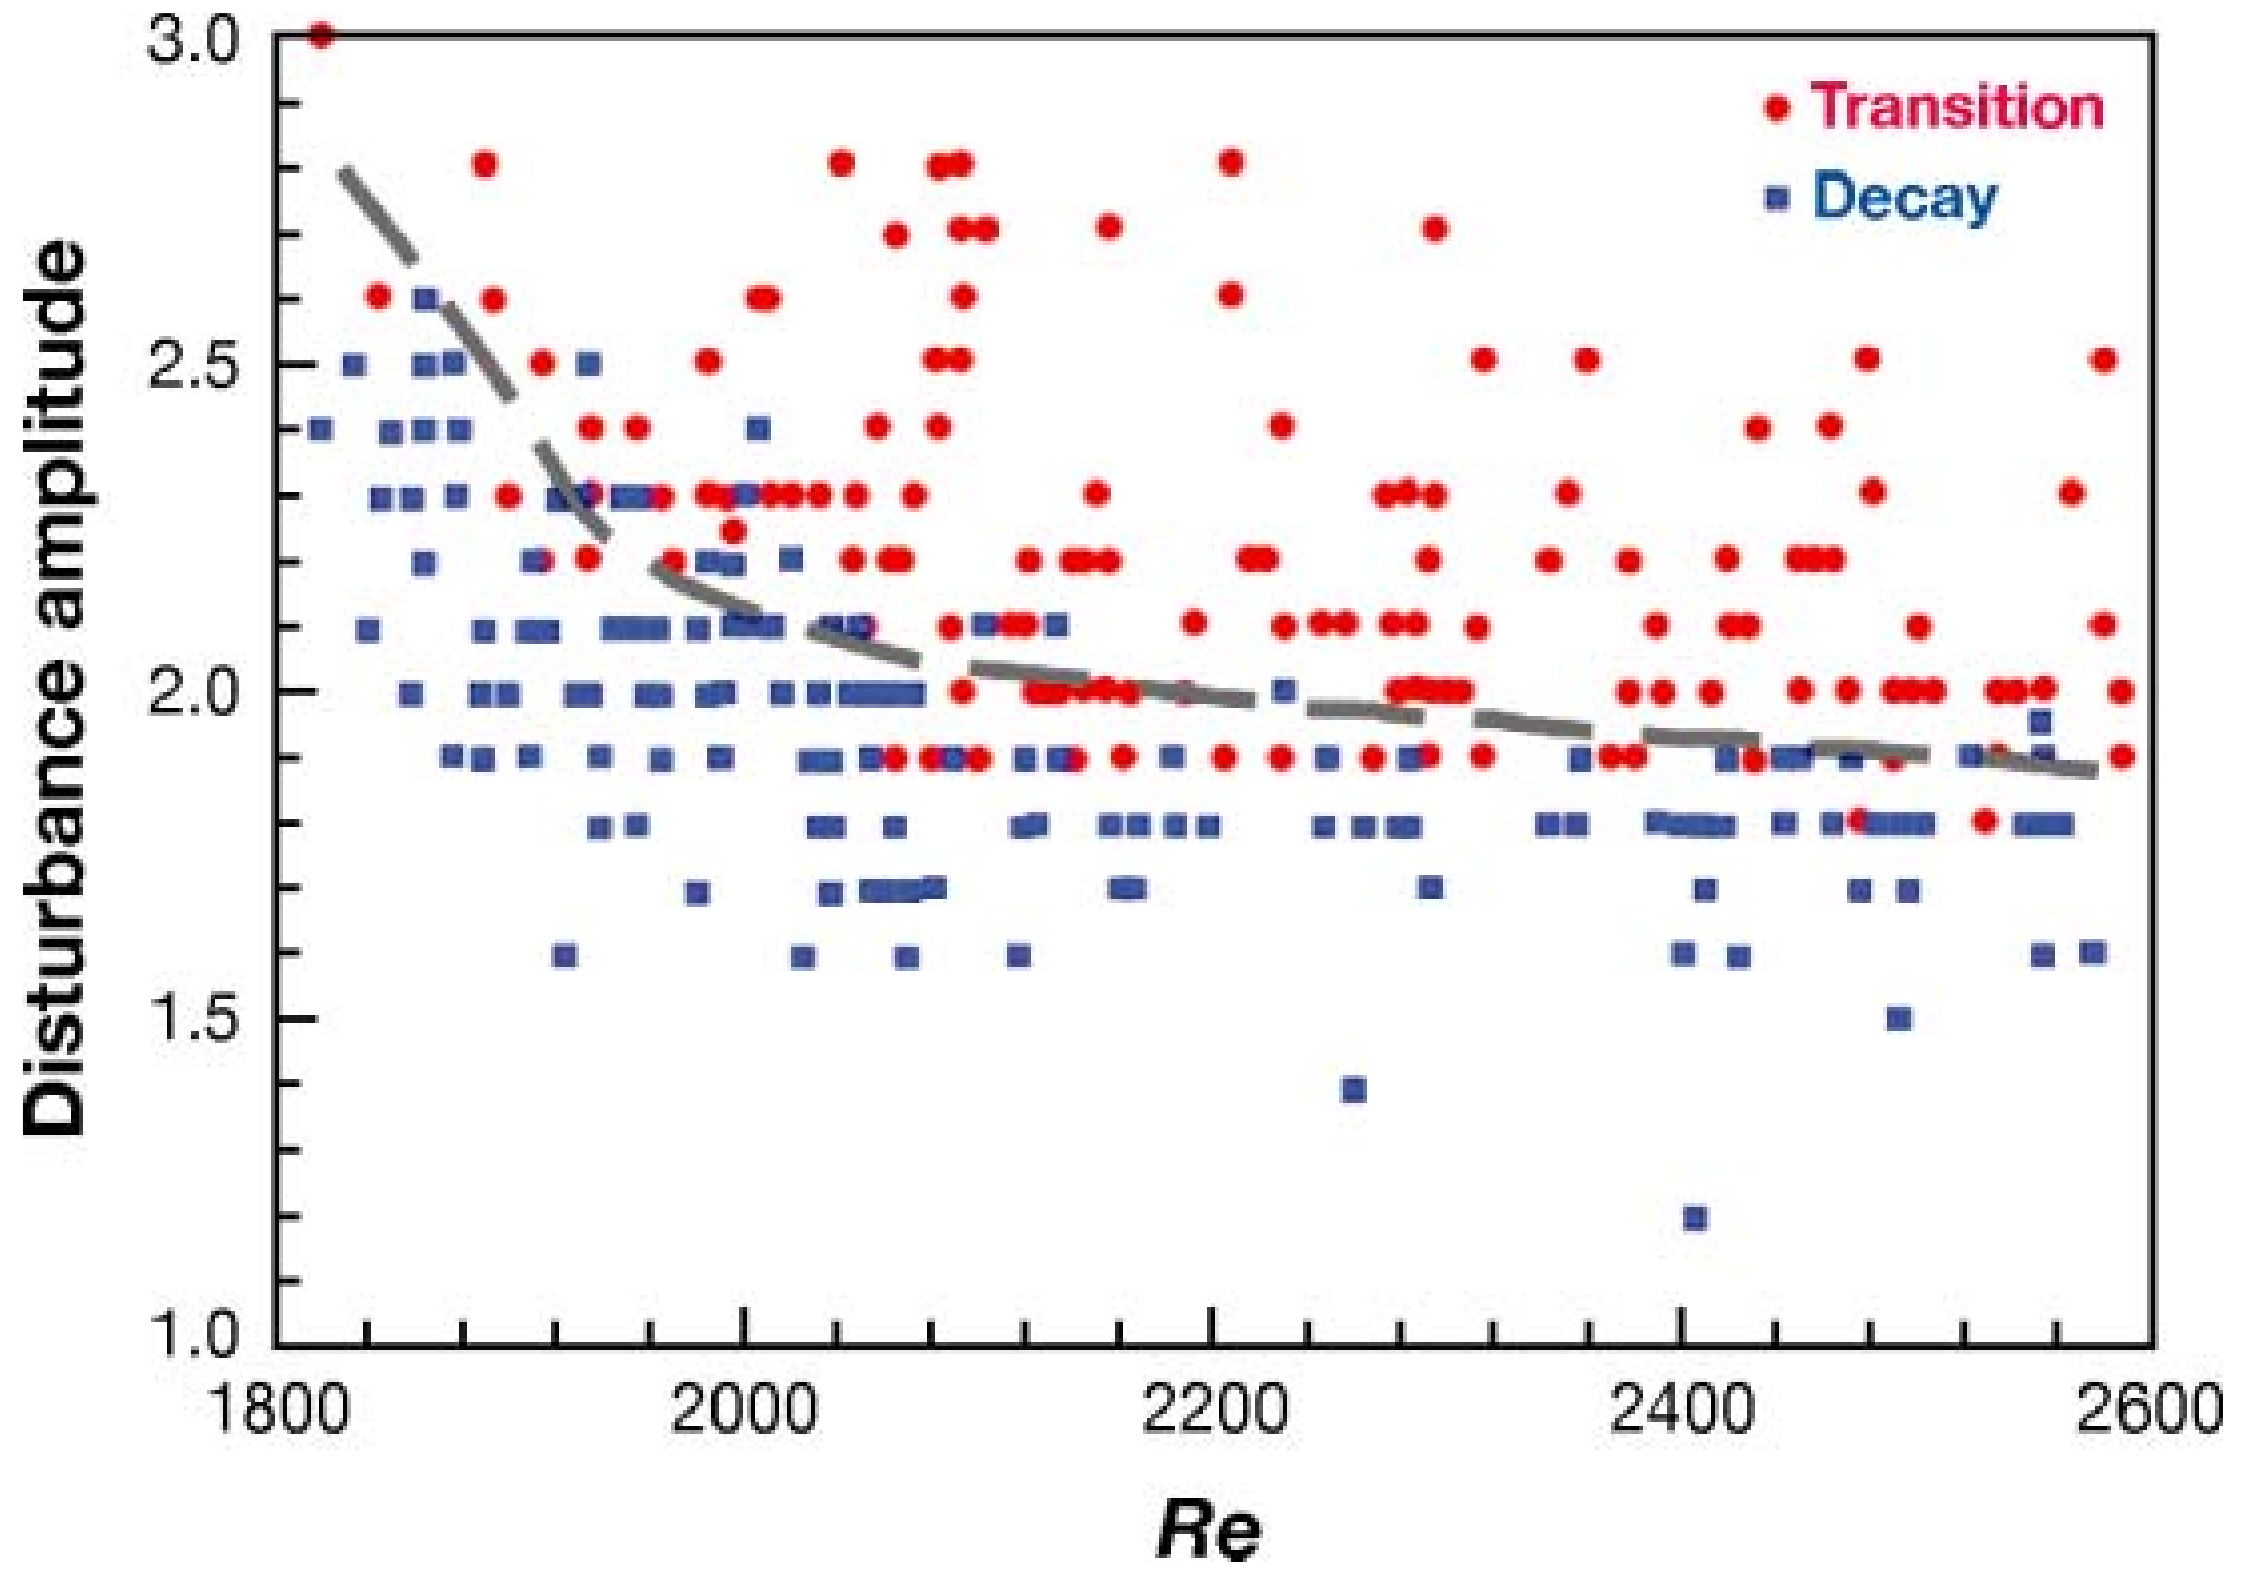
\includegraphics[width=0.95\textwidth]{darbyshire95.png}
    \caption{Turbulence transition results obtained by Darbyshire \& Mullin\cite{Darbyshire95}, reprinted and coloured by Eckhardt et al.\cite{Eckhardt07}}\label{img:darbyshire_plot}
\end{figure}

Despite that though, an approximate line can be drawn that separates the `mostly turbulent' area from the `mostly decaying' one and provides us with a relation that the higher the Reynolds number the smaller disturbance is required to trigger turbulence.
Of course this relation needs to be taken with a pinch of salt, as it is only correct on a coarse scale\cite{Eckhardt07}.
Any experiment has physical limits on its accuracy and so it is often only possible to use numerical simulations to investigate the effects of slight changes in starting conditions.
In a simulation one has perfect control (up to numerical accuracy and the algorithm chosen) over the starting conditions and the evolution of the simulation and thus much more accurate results are possible to be achieved.
In concert with the experimental results a simulation by Faisst \& Eckhardt\cite{Faisst04} shows that perturbation amplitudes very close to one another produce turbulence with strikingly different lifetimes.
Their results also confirm the inverse relation between the Reynolds number of a flow and strength of a perturbation required to trigger turbulence.
This relation is again confirmed by experiments in the ranges of Reynolds numbers from \(2000\) to \(20000\), where the `coarse-scale' critical amplitude dependence on \(Re\) as \(1 / Re\) is reported\cite{Hof03}\cite{Hof04}\cite{Draad98}.

\subsubsection{Lifetimes}
It is generally agreed that because of the strong variability of lifetimes with changing initial conditions, it is more useful to look at the lifetimes in bulk, focusing on certain statistical properties of them, such as the survival probability at different times from the instant when the perturbation was introduced.
Because of the positive Lyapunov constant in the evolution of the system through the phase space, the probability of decay to the laminar state is independent of time, just as in our example of a particle in a box.
Because of the decay probability being constant in time, the distribution of lifetimes is an exponential\cite{Kadanoff84}.
The experimental data confirms this theoretical prediction and exponential distribution of survival probability is indeed observed.
Such a distribution implies the earlier mentioned property of the turbulent state to be a chaotic saddle in the state space.
As well as being supported by experiment, numerical simulations also produce exponentially decaying survival probabilities\cite{Eckhardt02}.
Additionally, same functional form of the dependence was found in plane Couette flow by Bottin \& Chate\cite{Bottin98} experimentally, and numerically by Eckhardt\cite{Eckhardt02}.

\begin{figure}[h]
    \centering
    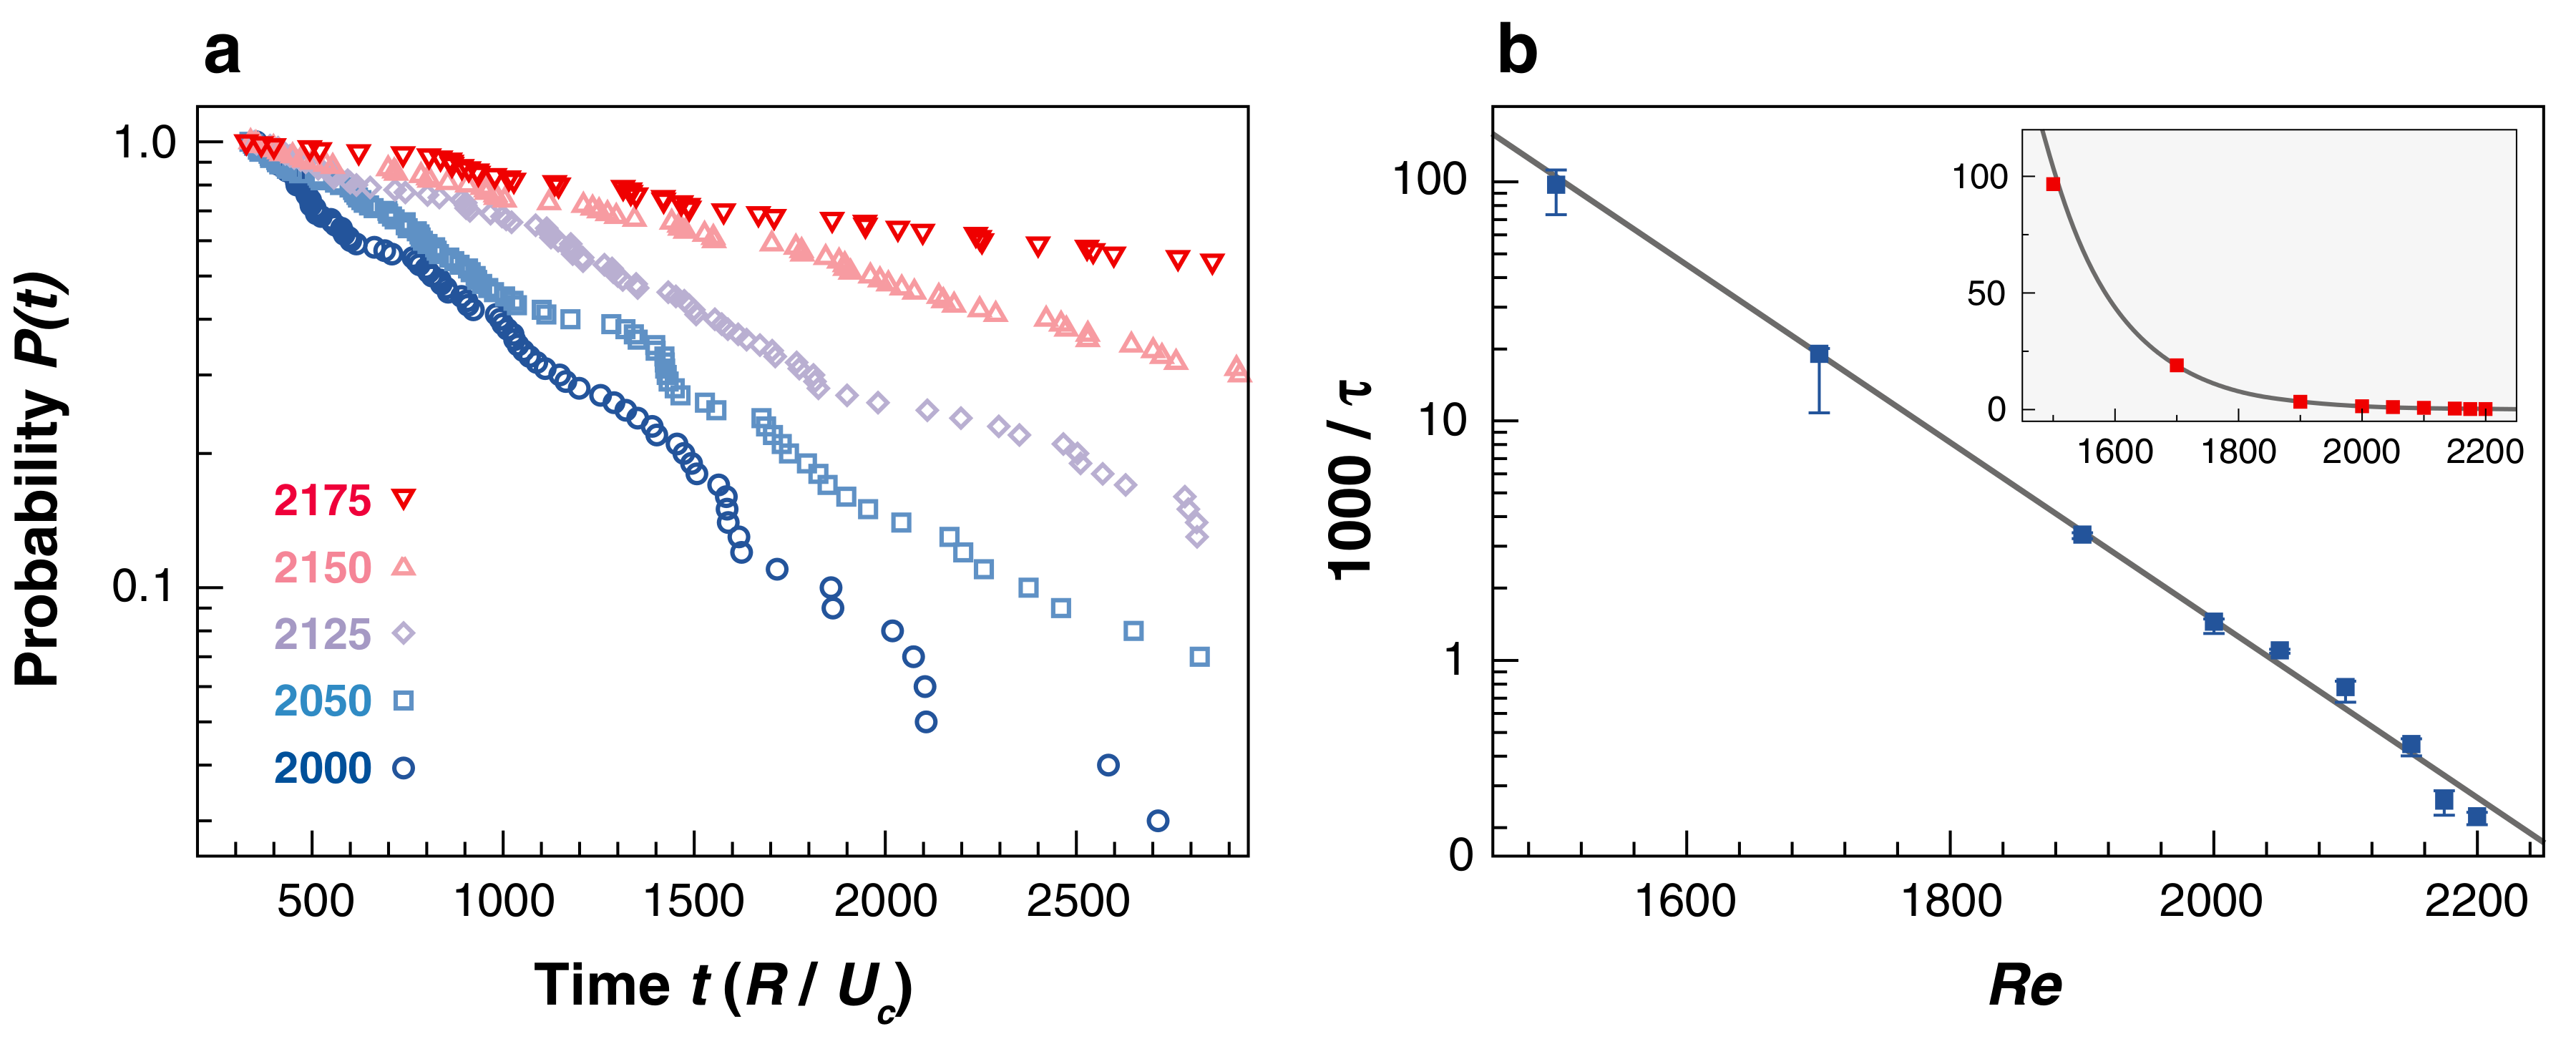
\includegraphics[width=0.95\textwidth]{decay_prob.png}
    \caption{Survival probabilities for different Reynolds numbers as determined by Direct Numerical Simulations by Eckhardt et al\cite{Eckhardt02}.}\label{img:decay_plot}
\end{figure}

Naturally, in the above cases we are talking about the tail of survival probability distribution, as at short lifetimes the evolution is influenced strongly by starting conditions and thus deviate from the exponential fit quite markedly in some cases.
Using the data we have from the numerical simulations we can tell that the characteristic time of the probability distribution increases quite drastically with an increasing Reynolds number.
While there is no theoretical prediction to the nature of the dependence of this time on the Reynolds number, the most recent experiments performed in long pipes suggest that the characteristic time does not diverge, but increases exponentially with Reynolds number.
This is in line with the results of numerical simulations which, in a limited \(Re\) range, have also shown an exponential increase of the characteristic time.

\subsubsection{Exact coherent states}
As much as the motion of a system in a turbulent state is chaotic, we know now that there exist simpler, regular solutions to the equations of motion.
Because we know that the turbulence is a chaotic saddle, different researchers have tried to find these saddle states around which the motion evolves\cite{Clever92}\cite{Clever97}\cite{Nagata90}\cite{Faisst00}.
Finding these states that guide the spatial and temporal evolution of a flow in a pipe may help with understanding the nature of flow better.
Because of the lack of inversion symmetry in the laminar profile of a pipe flow, the simplest coherent solutions to the equations of motion take form of travelling waves.
An example of such a travelling wave is presented on Image~\ref{img:stat_states}, arrows indicating fluid flow in place of the cross-section.

\begin{figure}[h]
    \centering
    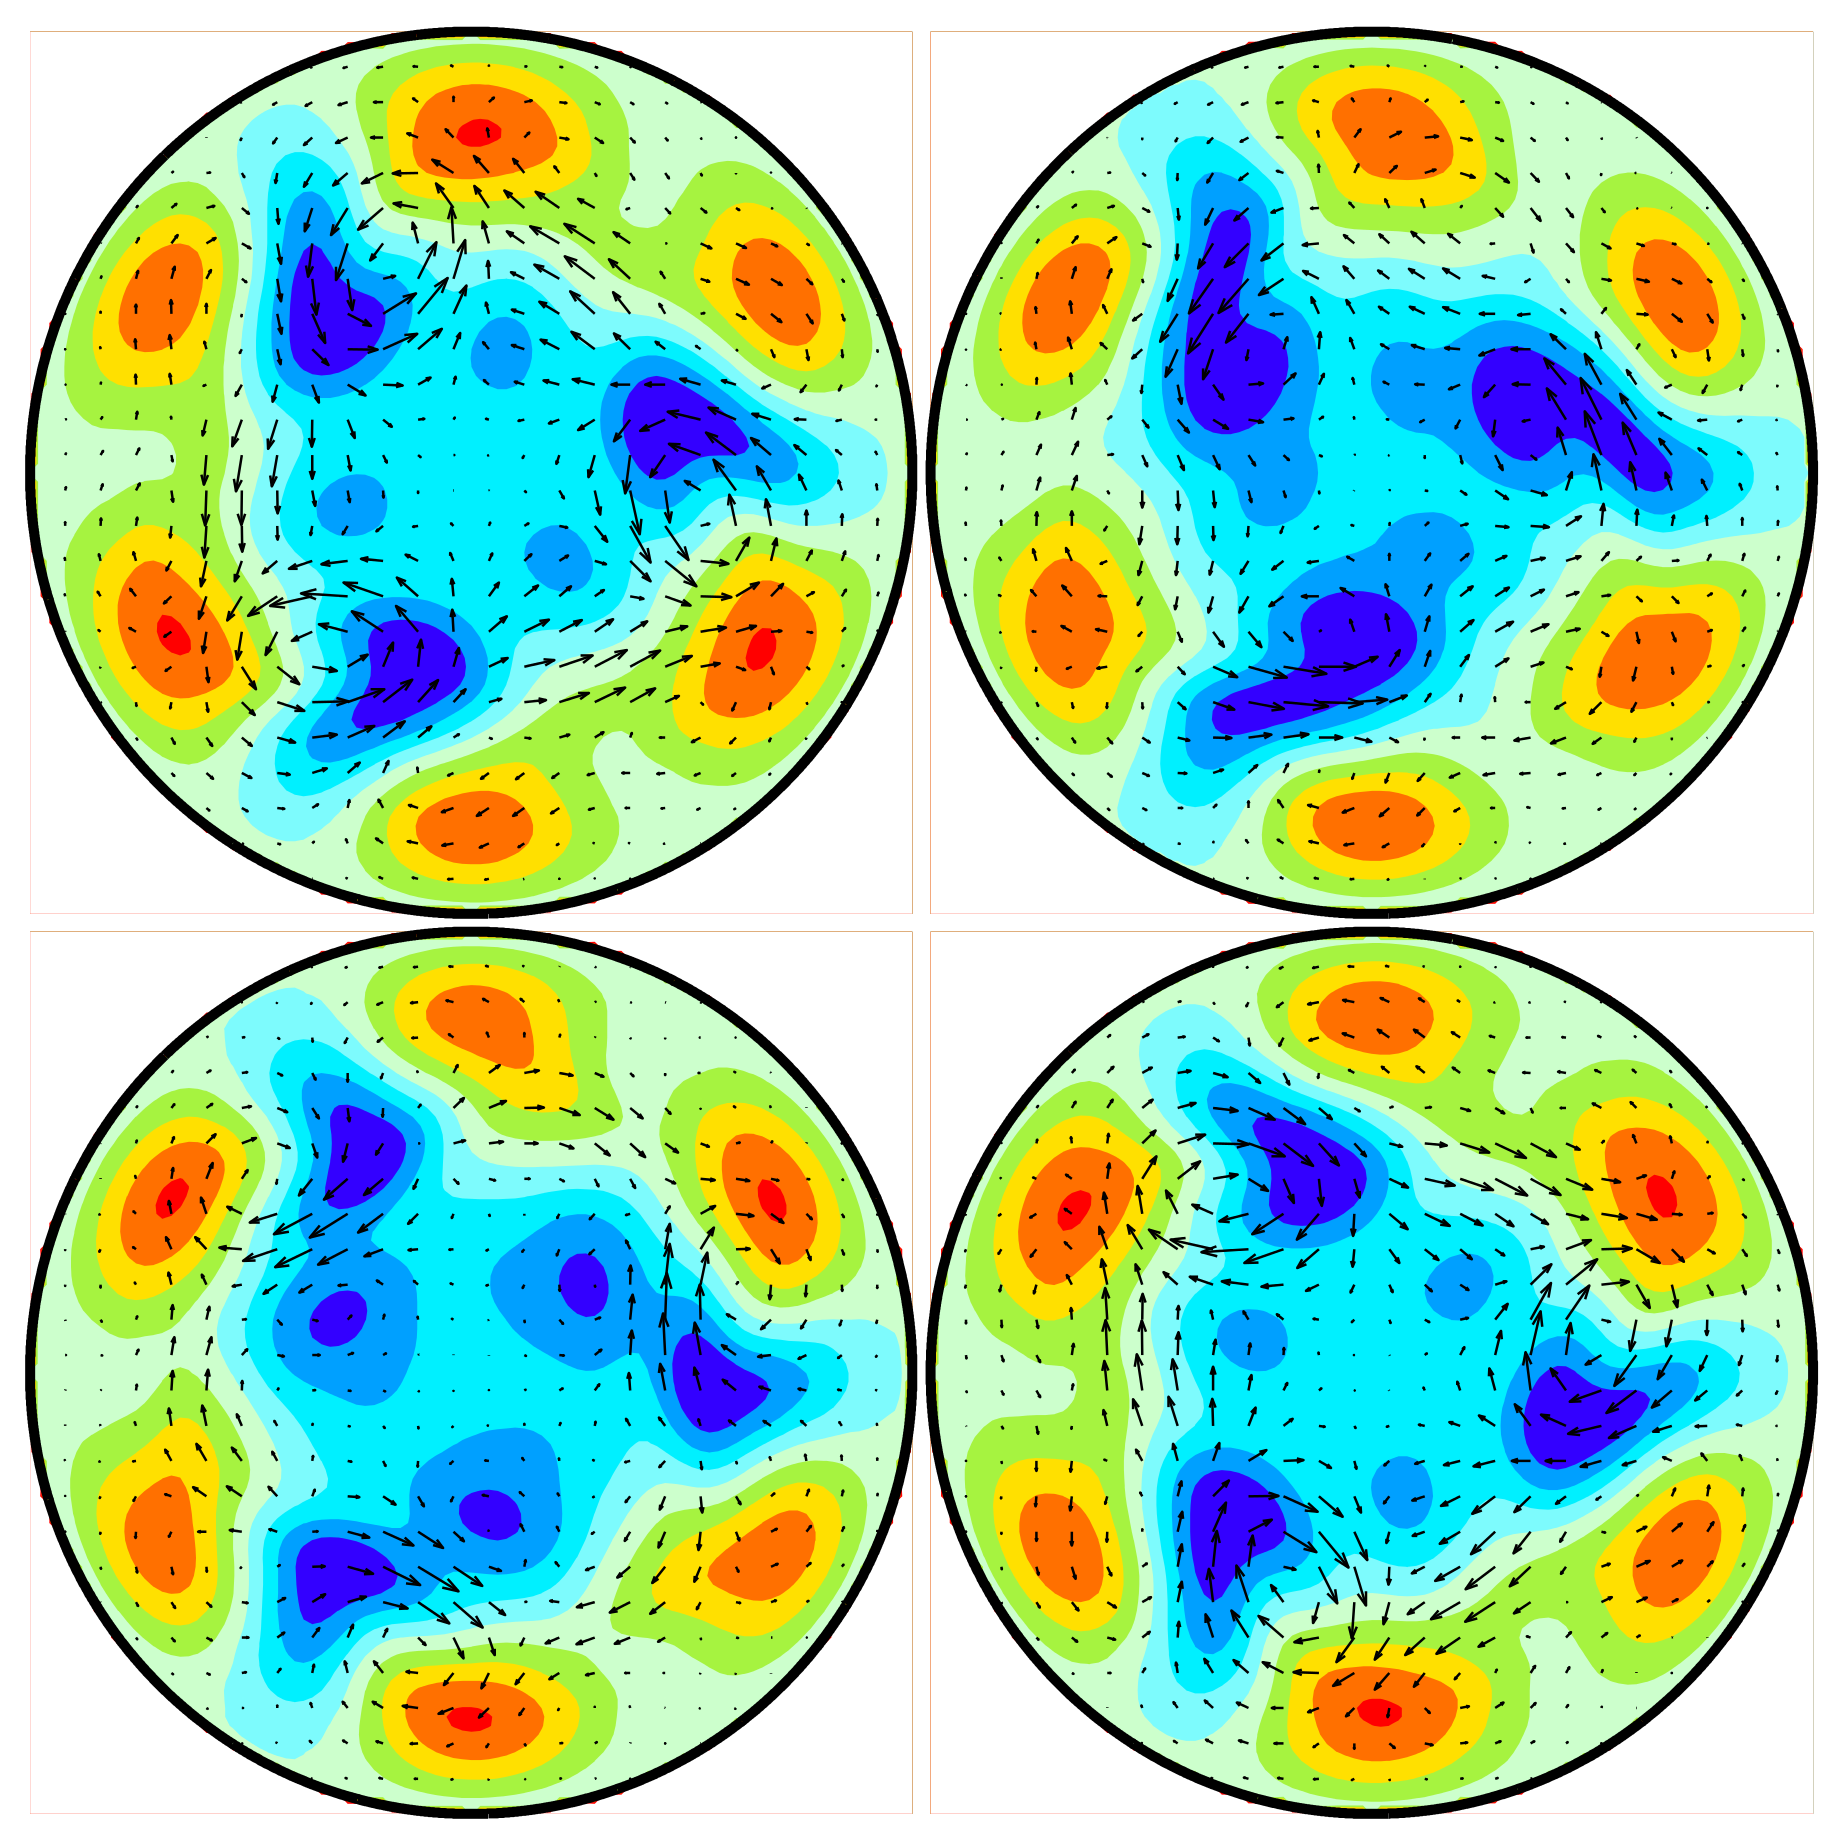
\includegraphics[width=0.65\textwidth]{stationary_states.png}
    \caption{An example of a stationary wave, shown here in the first half of its period (the other half is inverted in the horizontal axis). Each cross-section shows a snapshot of the wave every $1/6$ of its period, as found by Faisst \& Eckhardt\cite{Faisst08}.}\label{img:stat_states}
\end{figure}

The waves that have been found contain from two to five `vortex pairs that generate high-speed streaks close to the walls and low speed streaks in the centre'\cite{Eckhardt07}.
As the time passes, the high-speed streaks evolve very little, with some minor change in their intensity, whereas the low-speed ones move around the centre of the flow quite considerably.
States strikingly similar to the ones predicted by the simulation are observed by means of stereoscopic particle image velocimetry\cite{How04etal}.
The technique requires addition of light-reflecting particles and measuring their positions in a thin cross-section of the flow produced by light from a pulsed laser.
Difference between the observed states and the ones predicted by the simulation is due to both the dissipative nature of a flow and the fact that a trajectory of the system in a state space will lead close, but not through the stationary states.

An important idea to stress again is the fact that the survival probability for a chaotic saddle, such as the one spanned by the coherent state will be an exponential.
That, when one thinks about the analogy of particle in a box, implies that movement around a chaotic saddle will always decay, with a lower or higher component of an exponential.

\begin{figure}[h]
    \centering
    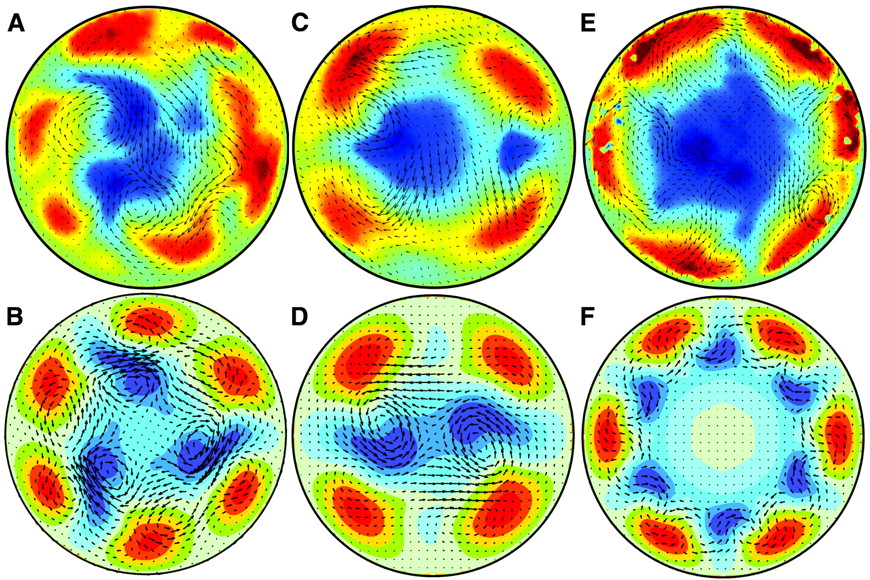
\includegraphics[width=0.95\textwidth]{experiment_vs_simulation.png}
    \caption{Comparison of the states predicted by the means of numerical simulation, on the bottom, and states observed with PIV\cite{Hof04etal}.}\label{img:ex_simu}
\end{figure}

\subsection{Drag reduction}

It turns out that addition of particles into the flow quite strikingly changes its behaviour and subsequent evolution in the state space.
It has been known since the 1940s\cite{Toms49}\cite{Mysels72} that addition of very limited amounts of polymers to water heavily reduces its its propensity to become turbulent and enables laminar flows at higher Reynolds numbers.
Additionally, once the motion becomes turbulent, the polymer additive reduces drag by around 80\%\cite{Sreenivasan00}.
Later it was noticed that elasticity displayed by the polymer is not required for a substantial modification of the flow dynamics\cite{Pashkewitz04} and materials such as paper or cloth pulp\cite{Radin75}\cite{Robertson57}, asbestos\cite{Mccomb85} and colloidal crystals\cite{Pirith72}\cite{Radin75}.
Drag reduction caused by the non-elastic additives is less pronounced than that caused by polymers of various kinds.
Even though certain methods have been proposed\cite{Pashkewitz04}\cite{Lee74} of combining properties of elastic and non-elastic additives to achieve stronger drag reduction, we will not discuss it here, as it is not a focus of this thesis.

This effect is widely applied in fluid transport in pipelines\cite{Graham04} and was considered to be used for faster sea transportation\cite{Dimotakis03}, before the idea was dropped because of costs concerns.
The reason why polymers were even considered to be worthy of being used in increasing speed of vessels on an open sea is that they are extremely potent drag reducers.
Even concentrations as low as parts per million produce visible effects.
An interesting property of the polymeric drag reduction is the existence of a phenomenon called the maximum drag reduction (MDR).
Once enough polymer is added to the solution, drag reduction can be observed.
As the concentration is increased, DR increases proportionally, until the point when it reaches a limit.
Adding more polymers cannot decrease the drag further.

\subsection{Motivation}
In this thesis we want to implement and test a simple, one dimensional model for turbulent flow and drag reduction in a pipe.
Because of a significantly reduced computational requirements, it is possible to execute the model for much longer times, domain sizes and numbers of runs than is possible with full direct numerical simulation of a fluid with embedded polymers.
We will compare the results produced by the model with the ones from both experiments and other numerical simulations to establish if the model correctly simulates real conditions in a fluid.
Because of certain limitations of the model discussed later it provides us with a limited set of information, though it should be enough for our needs.

\section{Introduction of equations}
In the subsequent thesis, we will focus on presenting a relatively simple system of coupled differential equations.
We will test if the system produces results that are in line with the large-scale behaviour of turbulent fluid in a pipe and thus will provide us with much more efficient model for analysing the flow than solving the full Navier-Stokes equation.
We feel that in presenting the equations it is much more educational to first consider the sources of our system of equations and then introduce the full system at the end.
This way the reader will gain an insight into rationale for existence of individual parts of the equations and will understand them on an intuitive level.

\subsection{Swift--Hohenberg equation}
In order to understand the dynamics of our system of equations~\eqref{eq:our1}, let's first consider a particular form of a Swift--Hohenberg\cite{Hohenberg74} equation, as presented in~\eqref{eq:sh1} (where $N(u)$ is some smooth non-linear factor proportional to $u^3$).

\begin{equation}\label{eq:sh1}
\frac{\delta u}{\delta t} = -\frac{\delta^4u}{\delta x^4} - 2\frac{\delta^2u}{\delta x^2} - (1 - \epsilon )u + N(u)
\end{equation}

As far as this equation does not simulate our turbulent system, it serves as a good basis for understanding of different issues that must be taken into account when creating a correct one.
One of the major requirements on a system of equations that would serve our purpose well is for it to exhibit chaotic behaviour.
To check if that is the case in~\eqref{eq:sh1}, let's think of a case of small perturbations, which lets us neglect the non-linear $u^3$ part and expand $u$ in Fourier modes. Then:

\begin{equation}\label{eq:sh_u}
    u \sim e^{\sigma t}e^{ikx}
\end{equation}

And expanding $\sigma$ in $k$ using~\eqref{eq:sh1} gives:

\begin{equation}\label{eq:sh_sigma}
    \sigma_{(k)} = -k^4 + 2k^2 - 1 + \epsilon = \epsilon - (k^2 - 1)^2
\end{equation}

Now we see that~\eqref{eq:sh_sigma}, substituted into~\eqref{eq:sh_u} gives the growth rate for an initial perturbation of a given frequency.
This is troubling, because it makes the time evolution linearly unstable.
To understand what this means, let's consider three possible cases.
If $\sigma_{(k)} < 0$ for a given $k$, it would imply that the disturbance of that frequency would decay towards zero because of the nature of exponential decay.
If $\sigma_{(k)}$ equals zero for a value of $k$, then this frequency would become constant and all the others would still decay.
In the last case of $\sigma_{(k)}$ being greater than zero for some values of $k$ we are faced with an exponential amplification of certain frequencies and decay of others.
This is not the desired dynamics at all -- we do not want en exponential explosion or decay.
We will have to modify the equation later to eliminate or counteract this property.

However, before we do that, let's focus on another of its troubling properties.
It can be proven\cite{Schneider96} that Swift--Hohenberg equation can be written in an Ginsburgh--Landau formalism, that is transformed in a way that would express the RHS in terms of a functional derivative:

\begin{equation}\label{eq:sh_landau}
    \frac{\delta u}{\delta t} = - \frac{\delta F[u(x)]}{\delta u(x)}
\end{equation}

As much as the repercussions of this fact may not be readily visible, let's consider computing the derivative of $F$, knowing~\eqref{eq:sh_landau}.

\begin{equation}\label{eq:sh_der}
    \frac{dF}{dt} = \int\frac{\delta F}{\delta u} \frac{\delta u}{\delta t}dx = -\int (\frac{\delta F}{\delta u})^2 dx
\end{equation}

Given that the term in the last equation is non-negative, the equation will follow the gradient of $F$ to minimise its free energy and present no chaotic behaviour.

\subsection{Kuramoto--Sivashinsky equation}
Continuing our journey of finding a suitable model to our problem, let's consider a slightly modified version of the above equation that is a special form of Kuramoto--Shivashinsky\cite{Hayman86} equation:

\begin{equation}\label{eq:ks1}
    \frac{\delta u}{\delta t} = -\frac{\delta^4 u}{\delta x^4} - 2\frac{\delta^2u}{\delta x^2} - (1 - \epsilon)u + u\frac{\delta u}{\delta x}
\end{equation}

This equation also exhibits a point of linear instability at $\epsilon = 0$.
It's behaviour is more interesting though, as if $\epsilon$ is just higher than zero, the solutions become periodic in time.
As $\epsilon$ is increased even further, the motion finally becomes chaotic.
Even though the motion is chaotic, it is at the same time linearly unstable.
In order to get rid of the linear instability we propose the following modification.

\subsection{Modified Kuramoto--Sivashinsky}
We require $\epsilon$ to be smaller then zero, to enforce linear stability.
Additionally, we note that if an amplitude in~\eqref{eq:ks1} is kept above a certain threshold, the chaotic behaviour is preserved.
In order to force the amplitude to remain in the chaotic region, we will couple our equation to a second one describing a field forcing the value of $u$.

\begin{equation}\label{eq:our1}
    \begin{split}
        \frac{\delta u}{\delta t} &= -\frac{\delta^4u}{\delta x^4} - 2\frac{\delta^2u}{\delta x^2} - (1 - \epsilon)u + u\frac{\delta u}{\delta x} + (1 - \epsilon)f(v)u \\
        \frac{\delta v}{\delta t} &= D\frac{\delta^2 v}{\delta x^2} - v + Ru^2 \\
        f(v) &= av + bv^2
\end{split}
\end{equation}

The above equation was first introduced by Becherer, Morozov and van Saarloos\cite{Morozov09}.
In~\eqref{eq:our1}, $a$ is larger while $b$ is smaller than zero.
This way, the amplitude of $u$ is forced to be around the zero of $f(v)$, while at the same time squashing the linear instability.
The equation for $v$ is rather simple, containing a diffusion term scaled by a constant $D$ and driving force proportional to $u^2$.
Both equations together are used by us to describe the evolution of decaying turbulence in a pipe filled with water.

In order to introduce polymers into the picture, we add an another coupled equation, to arrive at the following system of equations, with $f(v)$ of the usual form:


\begin{equation}\label{eq:our_poly}
    \begin{split}
        \frac{\delta u}{\delta t} &= -\frac{\delta^4u}{\delta x^4} - 2\frac{\delta^2u}{\delta x^2} - (1 - \epsilon)u + u\frac{\delta u}{\delta x} + (1 - \epsilon)f(v)u + \frac{\delta \tau}{\delta x}\\
        \frac{\delta v}{\delta t} &= D\frac{\delta^2 v}{\delta x^2} - v + Ru^2 \\
        \frac{\delta u}{\delta x} &= \tau + \lambda(\frac{\delta \tau}{\delta t} + u\frac{\delta \tau}{\delta x} - 2\tau\frac{\delta u}{\delta x})
\end{split}
\end{equation}

In~\eqref{eq:our_poly} $u$ is coupled to the $\tau$ field by its spatial derivative.
To understand the origin of the $\tau$ equation, let's consider a simplified system first, with $\tau$ equation substituted by:

\begin{equation}\label{eq:poly_simp}
    \frac{\delta u}{\delta x} = \tau + \lambda\frac{\delta \tau}{\delta t} 
\end{equation}

Here, the polymer field is composed of particles that relax exponentially (second term on the left).
The stretch is driven by spatial inhomogeneity of the $u$ field.
We feel that this is a viable assumption, as in a homogeneous velocity field no stretch caused by the velocity can happen, only translation of the polymers in space.

Now we can approach the full $\tau$ equation~\eqref{eq:our_poly}.
Let's consider the terms being multiplied by $\lambda$.
The second term from the left describes the advection of the polymeric stress with the flow of $u$.
It exists because we want the polymers to be able to be translated with the flow as they are diluted in it.The fourth term is related to polymeric normal stress, which reduces the value of $\frac{\delta u}{\delta x}$ proportionally to the polymeric stress.
% TODO: Write about this thing, why is the value reduced proportionally?

\section{Numerical methods}
Both~\eqref{eq:our1} and~\eqref{eq:our_poly} are highly non-linear systems of differential equations.
In order to solve them efficiently and accurately we use spectral methods\cite{Orszag80}, with dealiasing to get rid of the high-frequency noise.
We split the computation into two halves -- first we compute the linear part, then the non-linear one.
Because we use different numerical methods for each, such a split makes computations less expensive.
The reason for that will be explained in a few paragraphs.

The non-linear part is integrated with Euler method, with the step size sufficiently small to make errors acceptable.
Because computational complexity in calculating a convolution in a Fourier space is \BigO{n^2} and transforming back to real space (where convolution costs \BigO{n}) is \BigO{n\log(n)}, it is more efficient to compute the non-linear terms in the real space and then transform them back into the complex space to apply the linear propagation.

The linear part is solved using a Crank--Nicolson\cite{Crank47} method.
It is a combination of forward Newton method at time step $n$ and backward Newton at time step $n + 1$ for a given differential equation,  as follows:

\begin{equation}\label{eq:cn1}
    \frac{u^{n+1}_i - u^n_i}{\Delta t} = \frac{1}{2}[F^{n+1}_i(u, x, t, \frac{\delta u}{\delta x}, \frac{\delta^2u}{\delta x^2}, \frac{\delta^4u}{\delta x^4}) + F^n_i(u, x, t, \frac{\delta u}{\delta x}, \frac{\delta^2u}{\delta x^2}, \frac{\delta^4u}{\delta x^4})]
\end{equation}

For a differential equation of the form:

\begin{equation}\label{eq:cn_eq}
    \frac{\delta u}{\delta t} = F(u, x, t, \frac{\delta u}{\delta x}, \frac{\delta^2u}{\delta x^2}, \frac{\delta^4u}{\delta x^4})
\end{equation}

Notice that in order to obtain the value of $u^{n+1}$, a system of equations needs to be solved, as we do not know the value of $F^{n+1}_i$.
Because the split into the linear and non-linear parts is applied, $F$ is completely linear.
If it was not, it would be impossible to create a constant linear operator for the process and for each time step a non-linear system of equations would need to be solved, using Euler method.
This would substantially increase the length of the computations.
Thankfully for the computational effectiveness of the process, we split the equation and precompute linear operators can be precomputed ahead of time.
With operator precomputation, the computational complexity of propagating the equation to a new time step is \BigO{n}, with $n$ being the spatial resolution.
The advantage of Crank--Nicolson method over simple Euler scheme is drastically increased accuracy, as long as the ratio of $\Delta t$ to $\Delta x^2$ is kept low.

There is an additional problem that arises when~\eqref{eq:our_poly} is attempted to be solved.
Because $u$ and $\tau$ depend linearly on each other, a scheme that preserves causality needs to be employed.
A `simple' substitution of values of $u$ and $\tau$ into the equations would mix the time steps $n$ and $n+1$ with disastrous effects for correctness.
To see why, consider transforming the $\tau$ equation from~\eqref{eq:our_poly} in such a way as to put $\frac{\delta \tau}{\delta t}$ on LHS:

\begin{equation}\label{eq:tau_transf}
    \frac{\delta \tau}{\delta t} = \frac{1}{\lambda}\frac{\delta u}{\delta x} - u\frac{\delta \tau}{\delta x} - \frac{\tau}{\lambda} + 2\tau\frac{\delta u}{\delta x}
\end{equation}

Comparing with~\eqref{eq:our_poly} it can clearly be seen that $u$ linearly depends on values of $v$ and the other way around.
Given the above, we can write just the linear parts of $u$ and $\tau$ in the following form:

\begin{alignat}{2}
    \frac{\delta u}{\delta t} &= Lu + C\tau &\quad \frac{\delta \tau}{\delta t} &= Au + B\tau\\
    L &= -\frac{\delta^4}{\delta x^4} - 2\frac{\delta^2}{\delta x^2} - 1 + \epsilon & A &= \frac{1}{\lambda}\frac{\delta}{\delta x} \nonumber \\
    C &= \frac{\delta}{\delta x} & B &= - \frac{1}{\lambda} \nonumber
\end{alignat}

Substituting above into the Crank--Nicolson scheme:

\begin{equation}\label{eq:cn_ops}
    \begin{aligned}
        \frac{u^{n+1} - u^n}{\Delta t} &= L\frac{u^{n+1} + u^n}{2} + C\frac{\tau^{n+1} + \tau^n}{2} \\
        \frac{\tau^{n+1} - \tau^n}{\Delta t} &= A\frac{u^{n+1} + u^n}{2} + B\frac{\tau^{n+1} + \tau^n}{2}
    \end{aligned}
\end{equation}

Which can be written in a clear and readable matrix form:

\begin{equation}\label{eq:cn_simpl}
    \begin{aligned}
        \begin{pmatrix}
            u^{n+1} \\
            \tau^{n+1}
        \end{pmatrix} &= (I - Z)^{-1} (I + Z) \begin{pmatrix} u^n \\ \tau^n \end{pmatrix} \\
            Z &= \frac{\Delta t}{2}\begin{pmatrix}
            L & C \\
            A & B
        \end{pmatrix}
    \end{aligned}
\end{equation}

Because all the coefficients in the $Z$ matrix are constant, $(I - Z)^{-1}(I + Z)$ can be precomputed before integration.
This still results in \BigO{n^2} multiplications instead of \BigO{n} for each time step, but it is a cost that is not substantially higher (for typical number of dimensions) than that of other parts of the program.

\subsection{Starting conditions}
In order to integrate the equation~\eqref{eq:our_poly} numerically, we need to determine starting conditions.
As we are interested in the bulk behaviour of many turbulent runs and we need reasonable amount of statistics, we have decided to get the starting conditions from a random number generator.
We have chosen Mersenne--Twister\cite{Matsumoto98}, as it is very fast, has extremely large period, very good equidistirbution properties and is readily available on the platform used by us.
We seed the random number generator with a nanosecond--resolution timer, which ensures sufficient entropy in seed values, even if tens of thousands of programs are started at almost the same time.
As we do not need cryptographically--secure random numbers, the randomness offered by Mersenne--Twister is entirely sufficient to our needs.


\section{Results}
The results presented in this section were obtained on ARCHER, with $100000$ runs performed for each case.
As explained in more detail in Appendix~\ref{app:struct}, the fits are performed in Python using SciPy.
In order to estimate the intrinsic errors and get a better fit, multiple fits to a random sample of the tail of the survival probability distributions were performed.
Subsequently the values of resulting fit parameters were averaged and their variance was taken as a fitting error.
In every case discussed here the resultant errors are smaller than $1\%$ of the value of the function at a given point.
We decided not to include the error bars at the resultant plots, as they would be smaller than the width of the line used to draw the function, unnecessarily reducing the readability of the plots.
For the double exponential case the fits only succeeded when the number of maximum function calls of the fitting procedure was increased substantially to accommodate the high variability of the exponential function.

The data--gathering procedure was ran for the values of $R$ between $0.9$ and $1.09$ and domain sizes between $12\pi$ and $24\pi$, every $2\pi$ giving a total of 120 cases.
This gives a total of $12$ million runs, each taking an average time of 3 minutes will fully vectorised code.
The code was heavily optimised to exploit cache locality, automatic code vectorisation and large cache sizes of both AMD Interlagos (at HECToR) and Intel Ivybridge (at ARCHER) architectures.
As the result the performance of the numerical code was improved by more than $200\%$ from the initial average time for a run of 7 minutes in case of fluid with polymer.


\subsection{Survival probability}
As was established in the theoretical introduction, the decay probability of a chaotic system should be constant in time.
This is caused by a chaotic saddle structure coupled with a Lyapunov constant of the motion.
Just as in an example of a particle bouncing in a non-uniform box with a hole, the survival probability of the motion inside the chaotic box should quickly become exponential.
As can be seen on Figure~\ref{img:surv_prob}, our system exhibits the same behaviour.

\begin{figure}[h!]
    \centering
    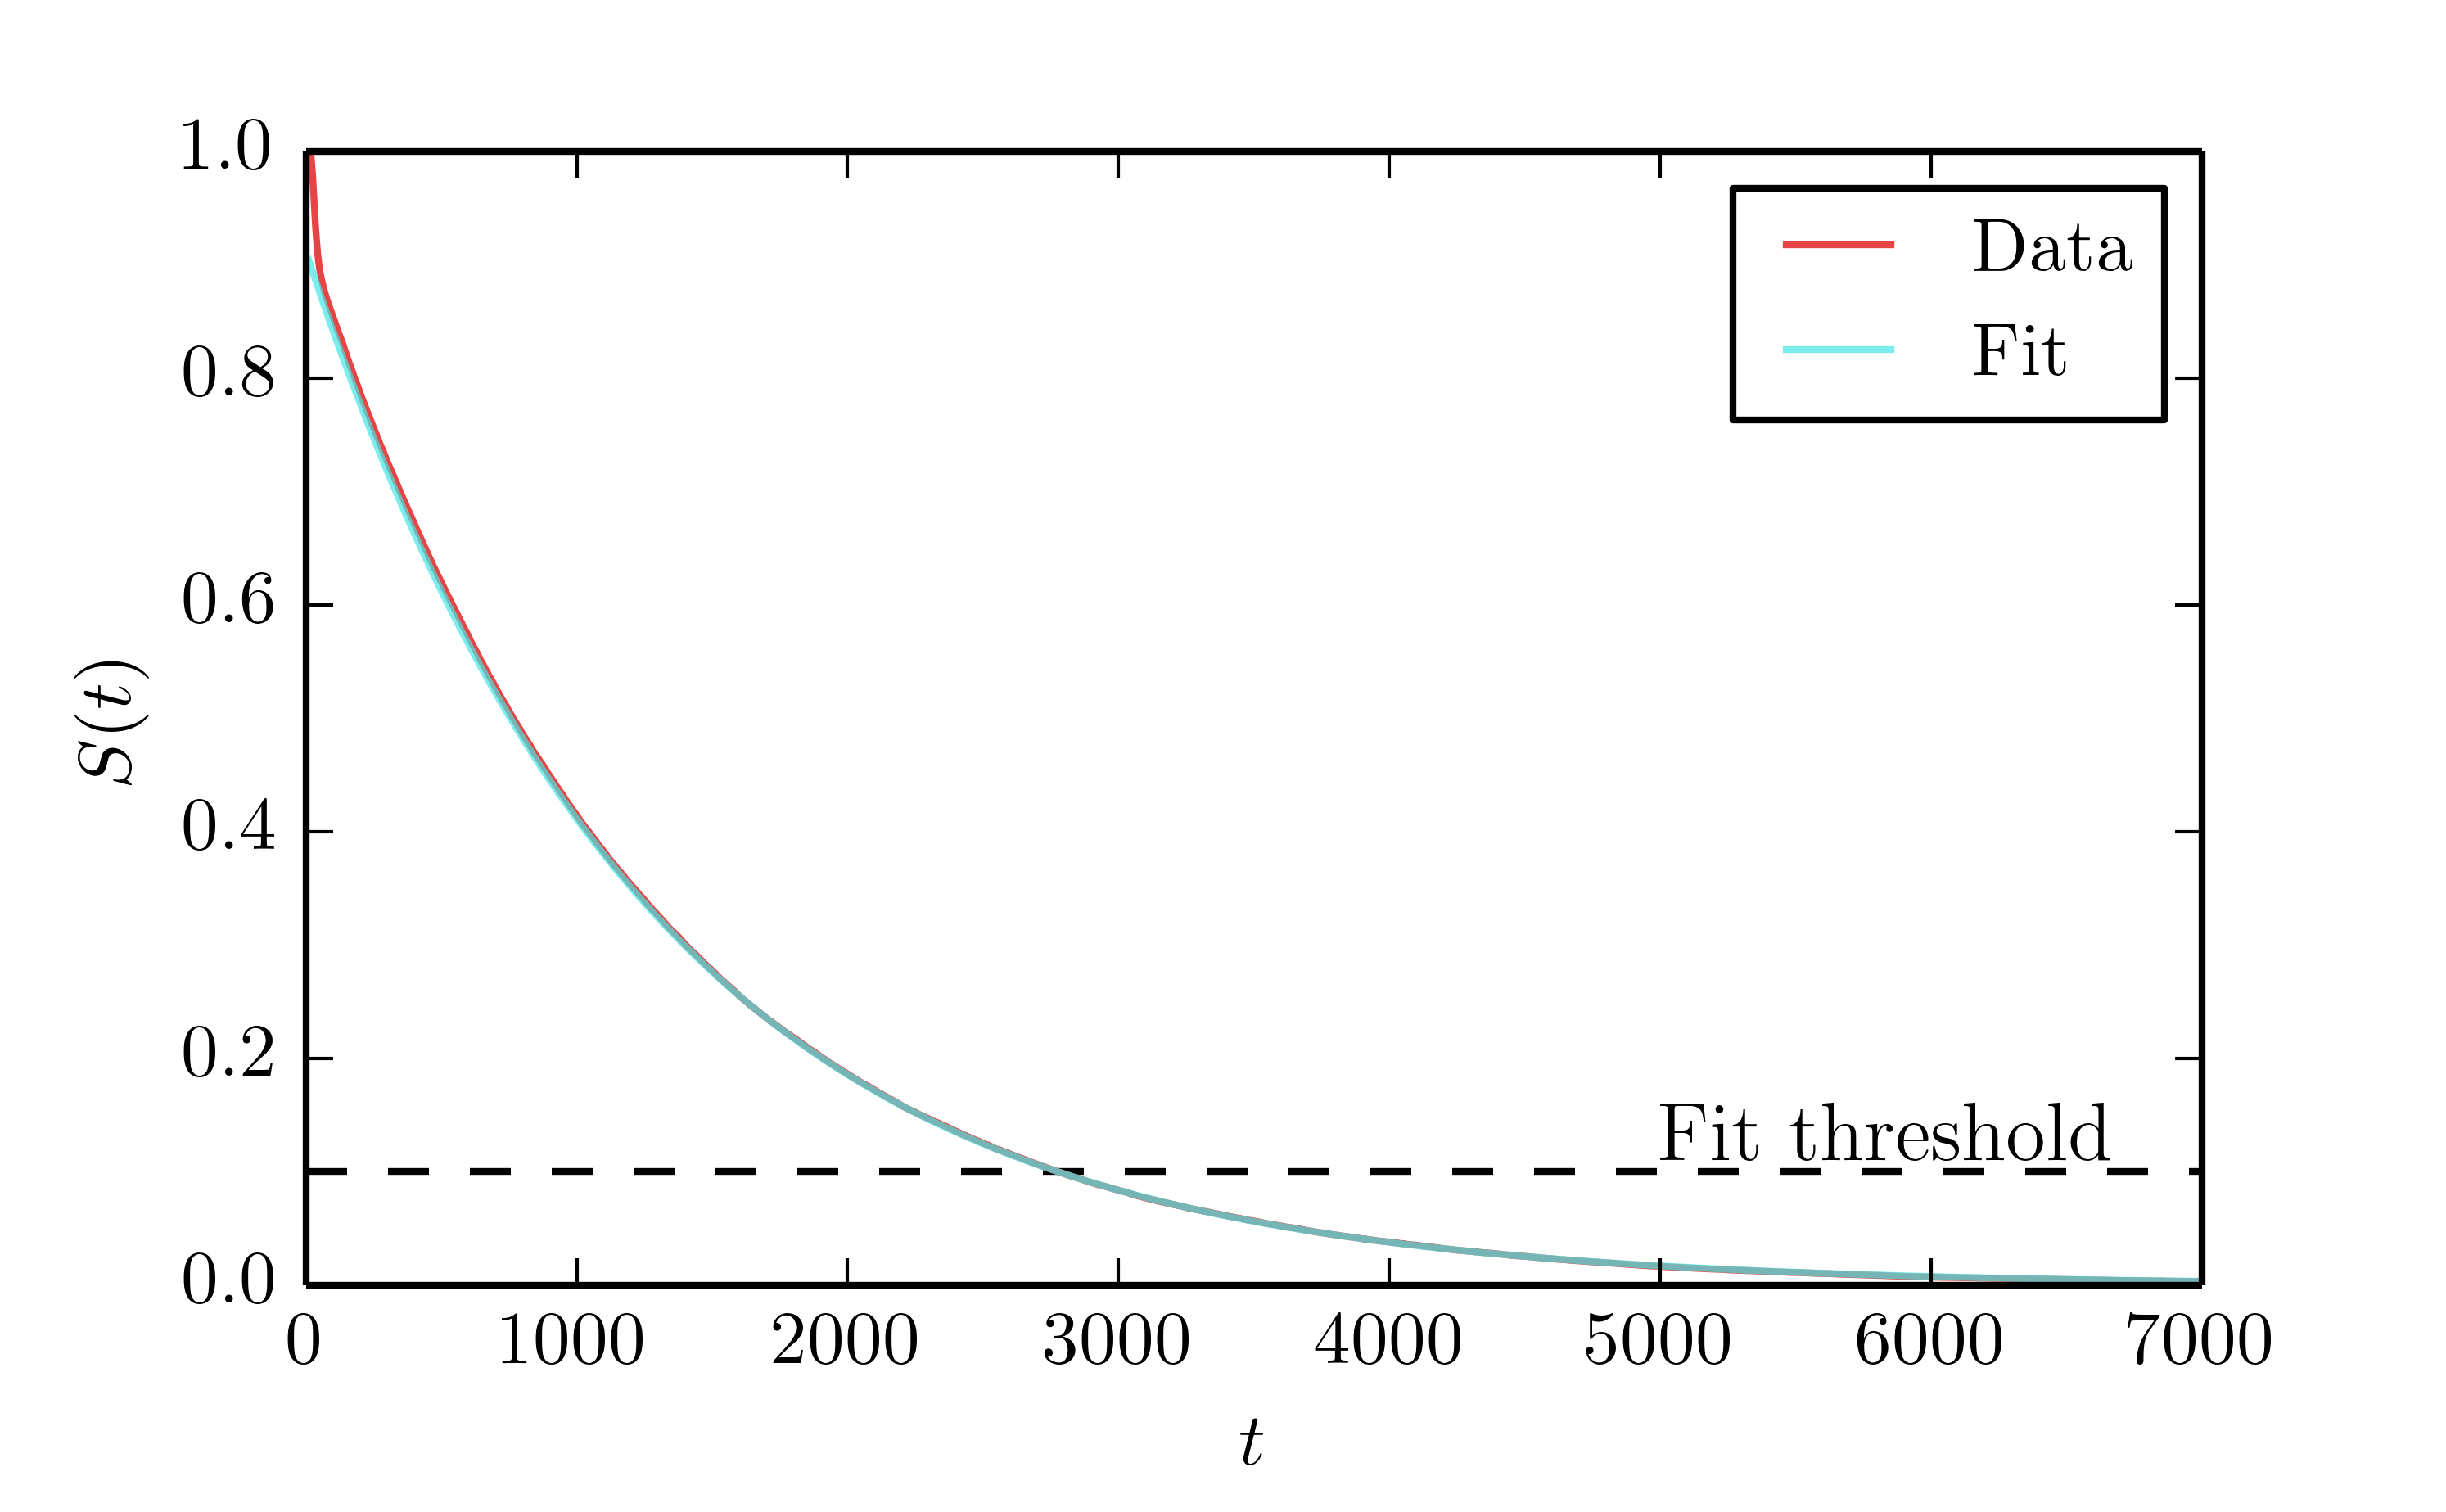
\includegraphics[width=\textwidth]{surv_prob.png}
    \caption{Survival probability of turbulent motion for $R=1.06$ with an exponential fit to the data. The threshold below which the points are fitted to the function is presented for easy visualisation.}\label{img:surv_prob}
\end{figure}

The data is fitted to an exponential function of the form:

\[ f(t) = a_0 e^{a_1t}\]

The fit to the tail of the data distribution is extremely precise, except possibly at the beginning of the distribution where the deviation is caused by the dependence on the initial conditions before the Lyapunov exponent takes over.
The maximum time of the simulation was not constant, as $a_1$ depends strongly on the value of $R$.
Therefore to achieve good fitting results it was increased for $R > 1.06$ to $21000$, which caused subsequent fits to be much more accurate.

An interesting intuitive parallel can be drawn between the appearance of this graph and the survival in radioactive decay.
The functional behaviour of the fit of the turbulent decay data is the same as the survival probability of a radioactive decay.
This correlation stems from the constant decay probability of a chaotic saddle and radioactive decay, which again confirms the assumption for the motion simulated by our equation follows that observed in experiments in turbulence.


\subsection{Double exponential fit to the values of $a_1$}
To verify that our system of equations simulates real turbulence well, we require two effects to be present.
First of all, in line with the experimental literature~\cite{Hof06}, we expect $a_1$ to depend double exponentially on the values of $R$.
It is a very delicate test and if it is possible to validate it will provide a strong validation to our model.
Additionally, we predict that the lower the domain size the less strong the dependence of $a_1$ is going to be on the Reynolds number.
We think that this will occur because as we reach the Minimal Flow Unit, the behaviour of the fluid becomes more and more simple thus leaving less possibility of variation with the increasing $R$.
To test the first hypothesis, we've attempted a fit to a double exponential function of the following form:

\begin{equation}\label{eq:g}
 g(R) = b_0\exp(-b_1\exp(b_2R))
 \end{equation}

We managed to obtain a good quality fit for all domain for which data is present except $14\pi$.
Because the double exponential fit is so dependent on starting conditions it is possible that a different choice of those would create a viable fit for that domain size.
The lack of convergence of the fitting procedure for $14\pi$ is not an important issue though, as we have a wealth of other measurement points.
For domain sizes other than $14\pi$ the fits of good quality are possible.

When it comes to accuracy of the fit, we expect some loss of accuracy as $R$ increases.
This is caused both by possibly insufficient maximum fitting simulation runtime and just lower amount of points in the distribution available at higher run times.
Unfortunately, it was impossible to increase the maximum time further than $21000$, as our runtime quota on ARCHER was saturated before we noticed the inadequate runtime.

\begin{figure}[h!]
    \centering
    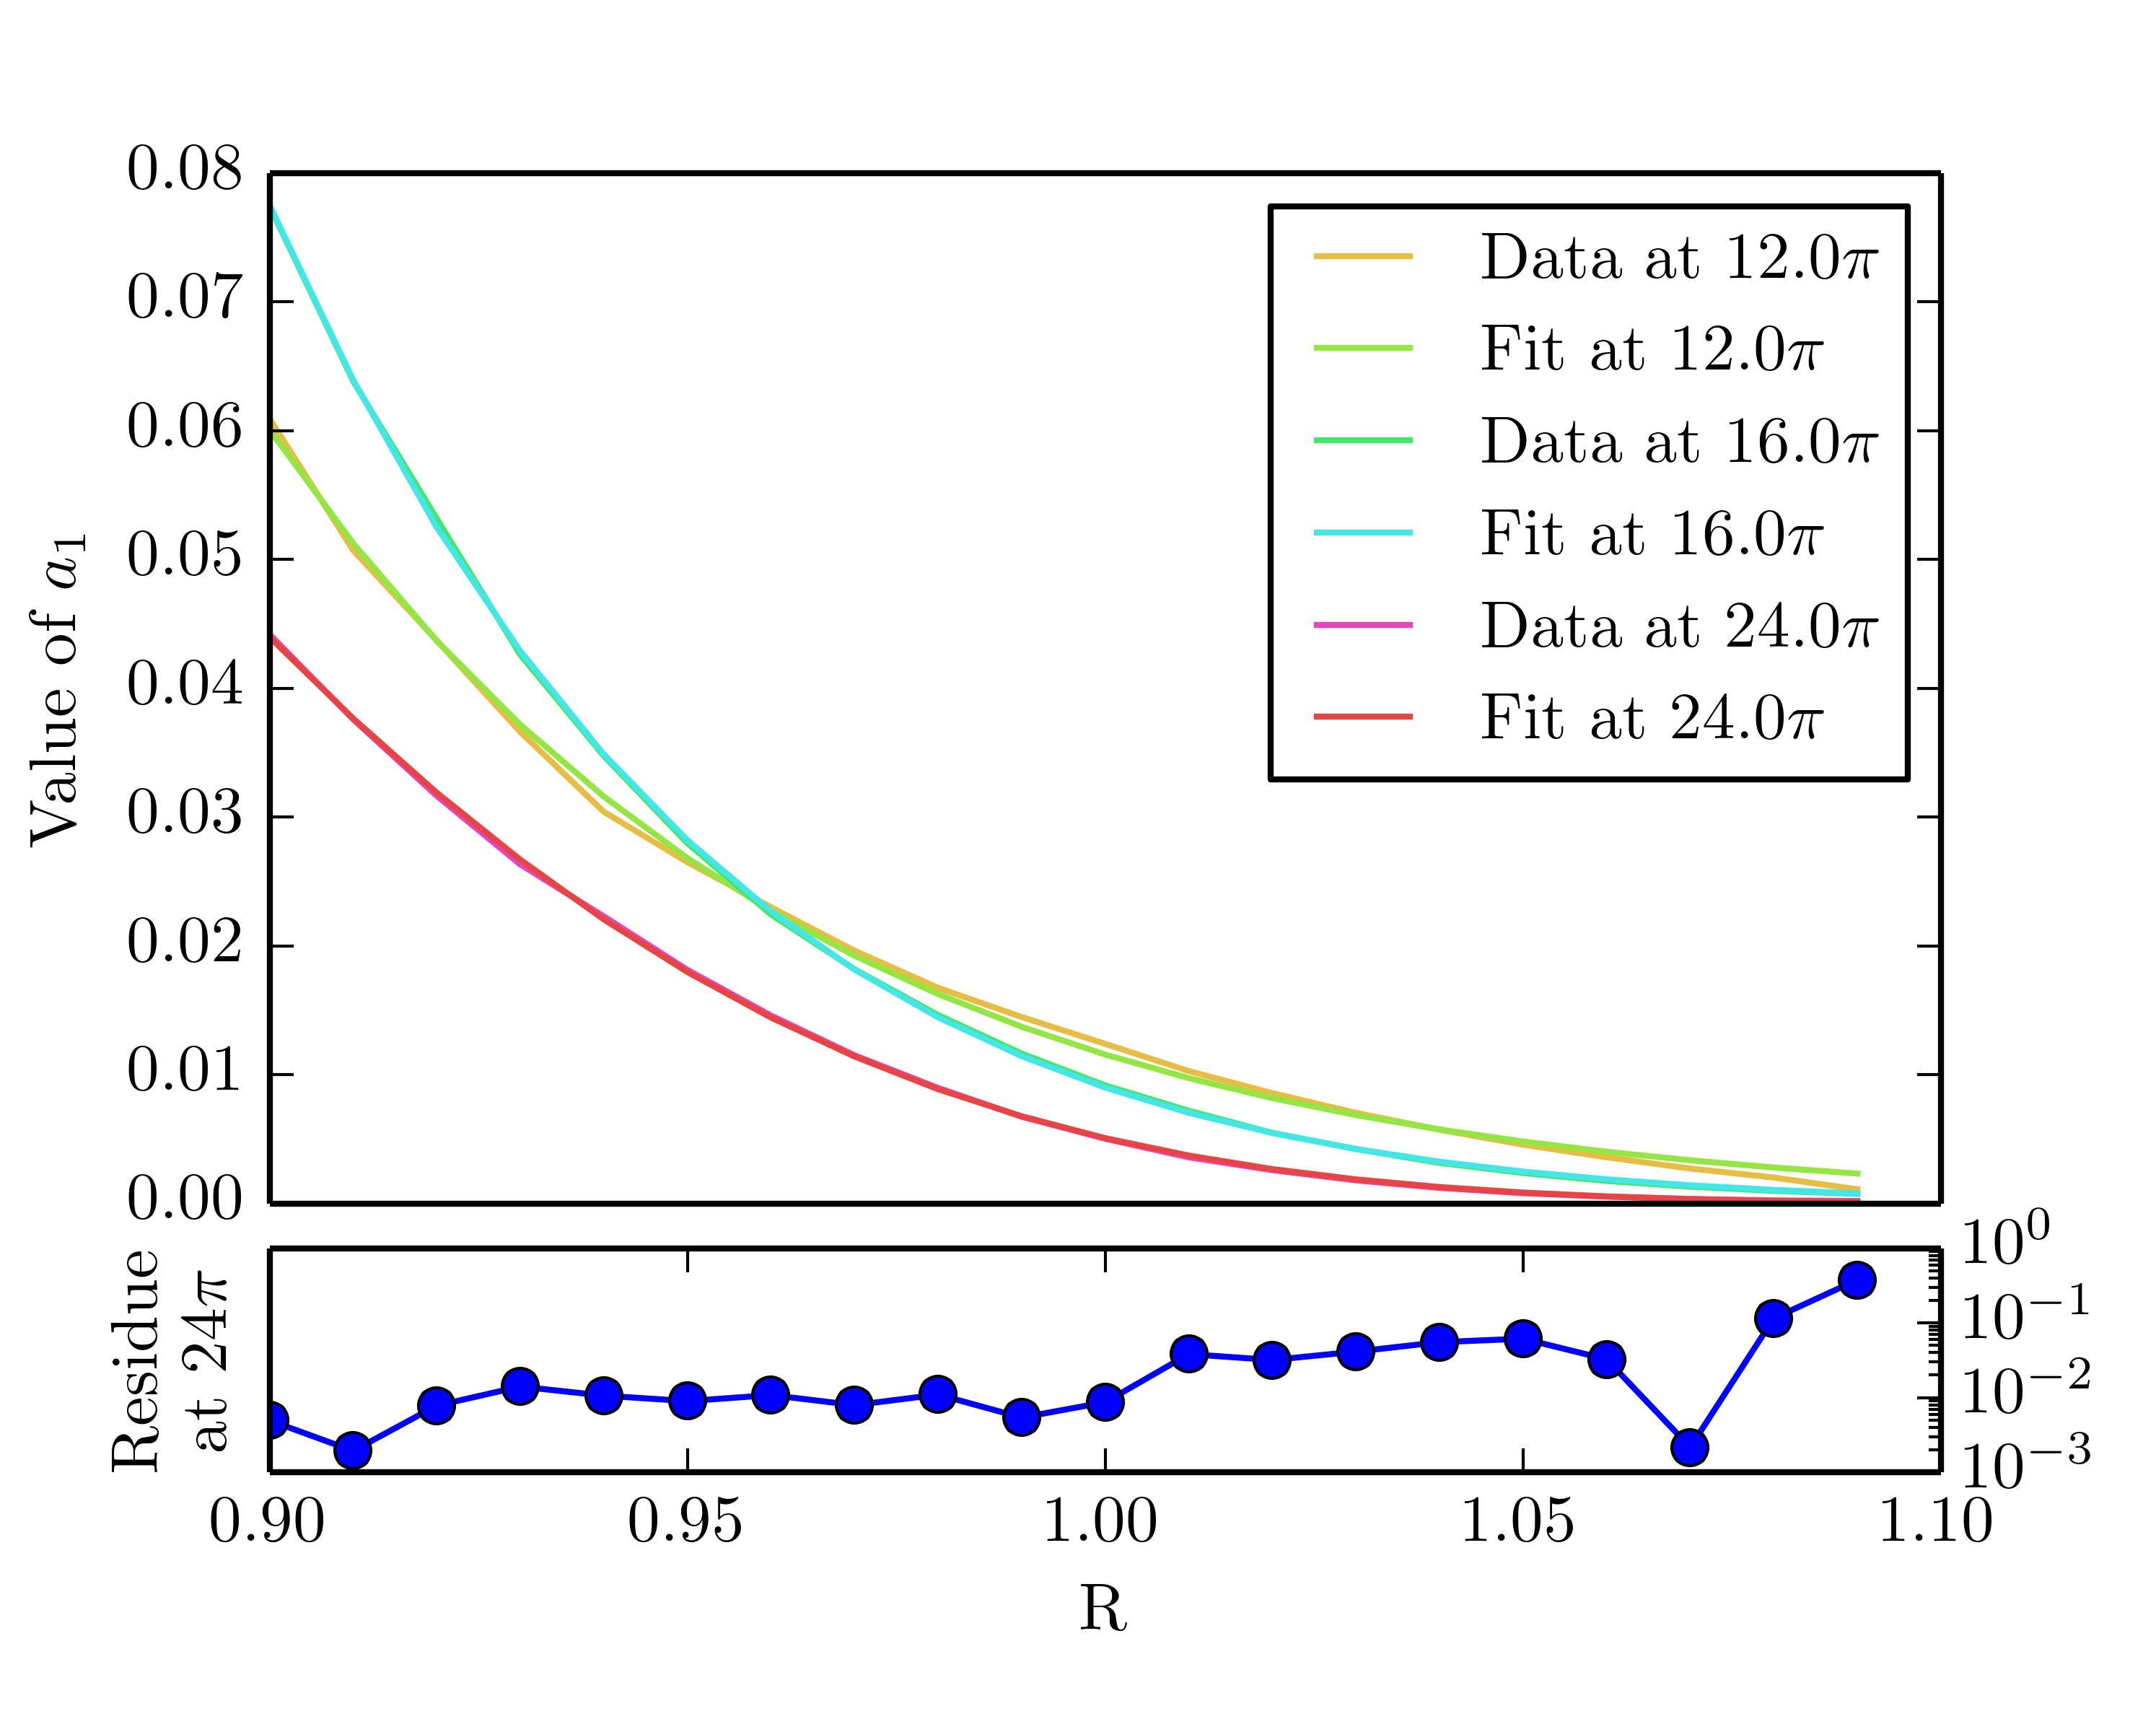
\includegraphics[width=\textwidth]{double_exp_fit}
    \caption{Values of $a_1$ at selected domain sizes and a double exponential fit to them (top). The bottom shows the fit residue at the highest domain size divided by the value of the data at a given data point.}
\end{figure}

The dependence of the fit parameters on the domain size is presented on Figure~\ref{img:b_params}.
It is interesting to notice that as $b_1$ decreases exponentially, $b_2$ increases almost linearly.
This begs the question, if the values of $g(x)$ intrinsically different for various domain sizes beyond a scaling factor.
It is possible for the effects of $b_1$ and $b_2$ to completely cancel themselves and then the only difference between them would be a scaling factor.

\begin{figure}[h!]
    \centering
    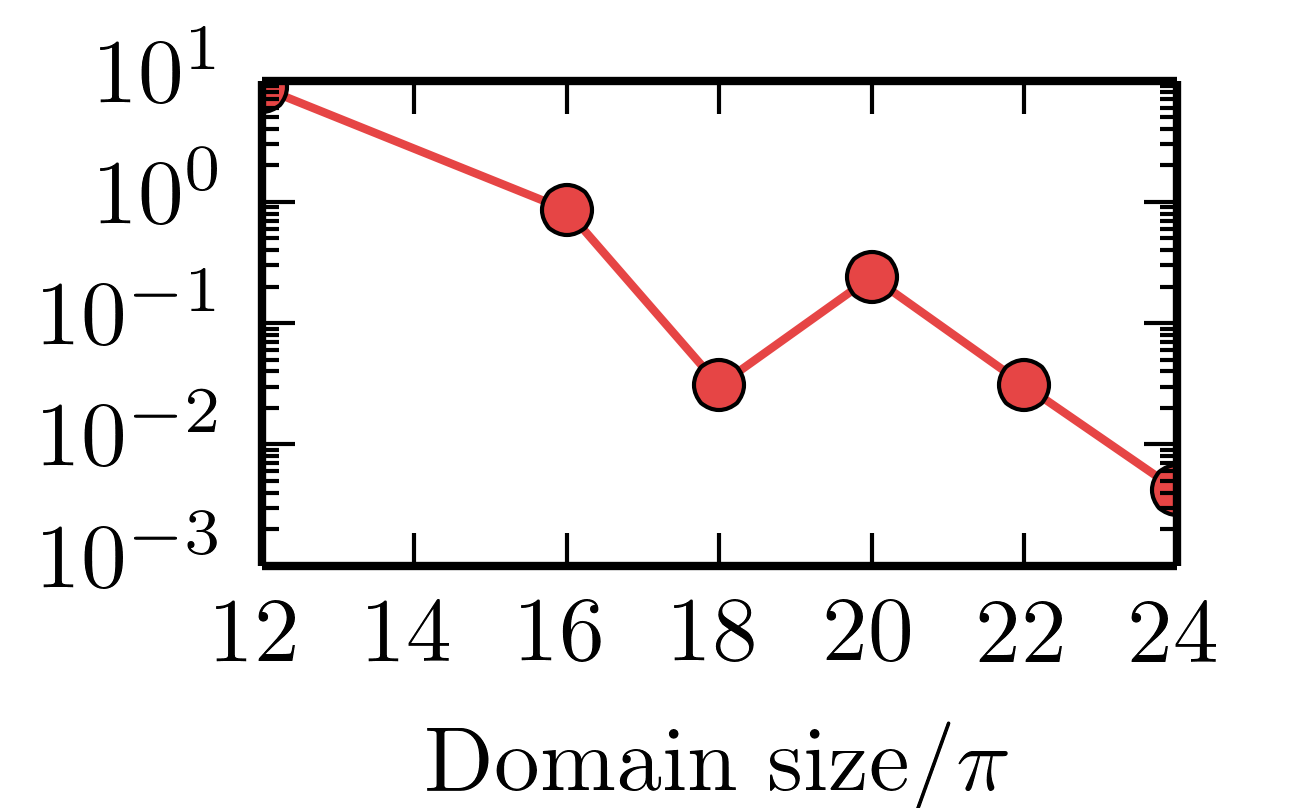
\includegraphics[width=0.45\textwidth]{b1_vs_domain.png}
    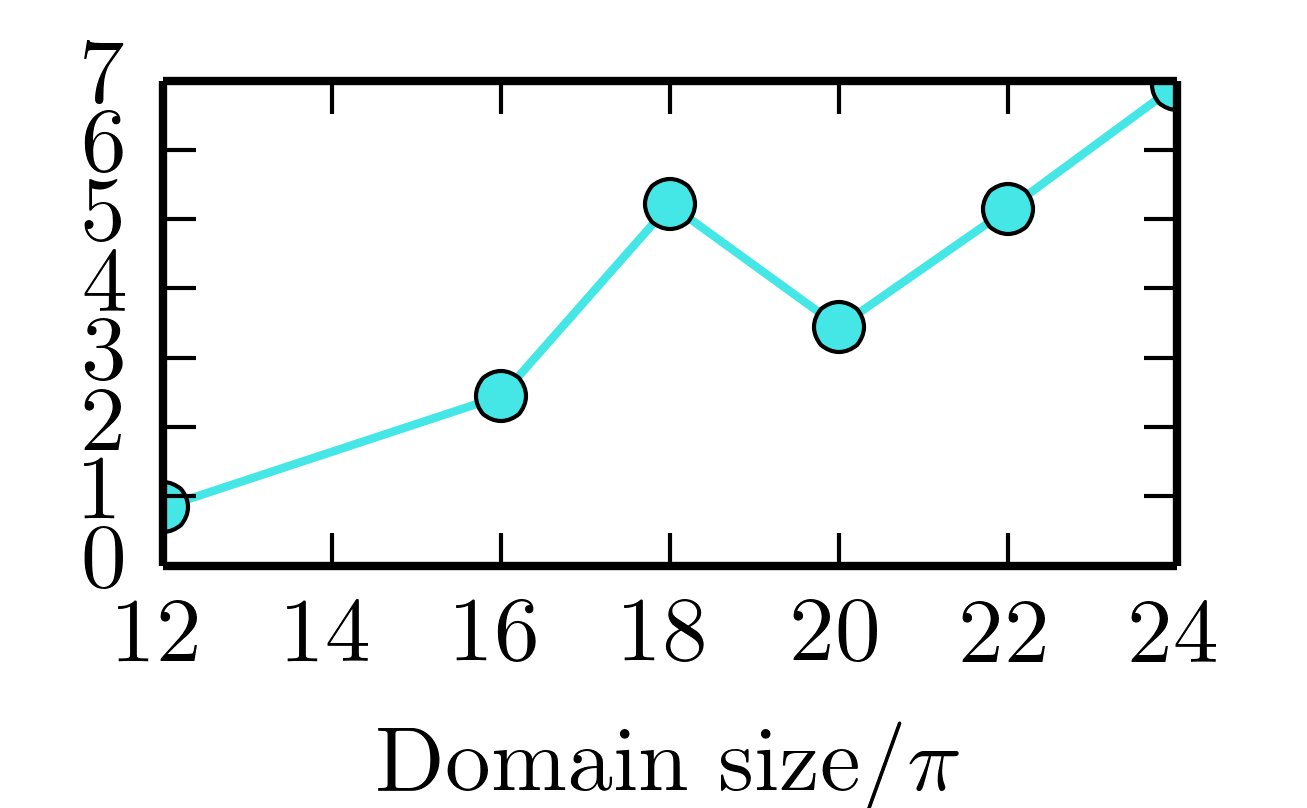
\includegraphics[width=0.45\textwidth]{b2_vs_domain.png}
    \caption{The double exponential fit parameters $b_1$ (left) and $b_2$ (right) for domain sizes for which a fit was possible to be constructed.}\label{img:b_params}
\end{figure}

We can infer some general qualitative information regarding this problem from the already presented plots.
Even from that limited data it seems that the dependence is deeper than just the effect of a scaling factor, for instance $12\pi$ overtakes $16\pi$ for large $R$.
In order to gain more insight, let's consider the second derivative on Figure~\ref{img:2der}.
Our expectation is for the second derivative to increase as the domain size grows.
This would mean that as the domain size increases the motion depends more strongly on $R$.

\begin{figure}[h!]
    \centering
    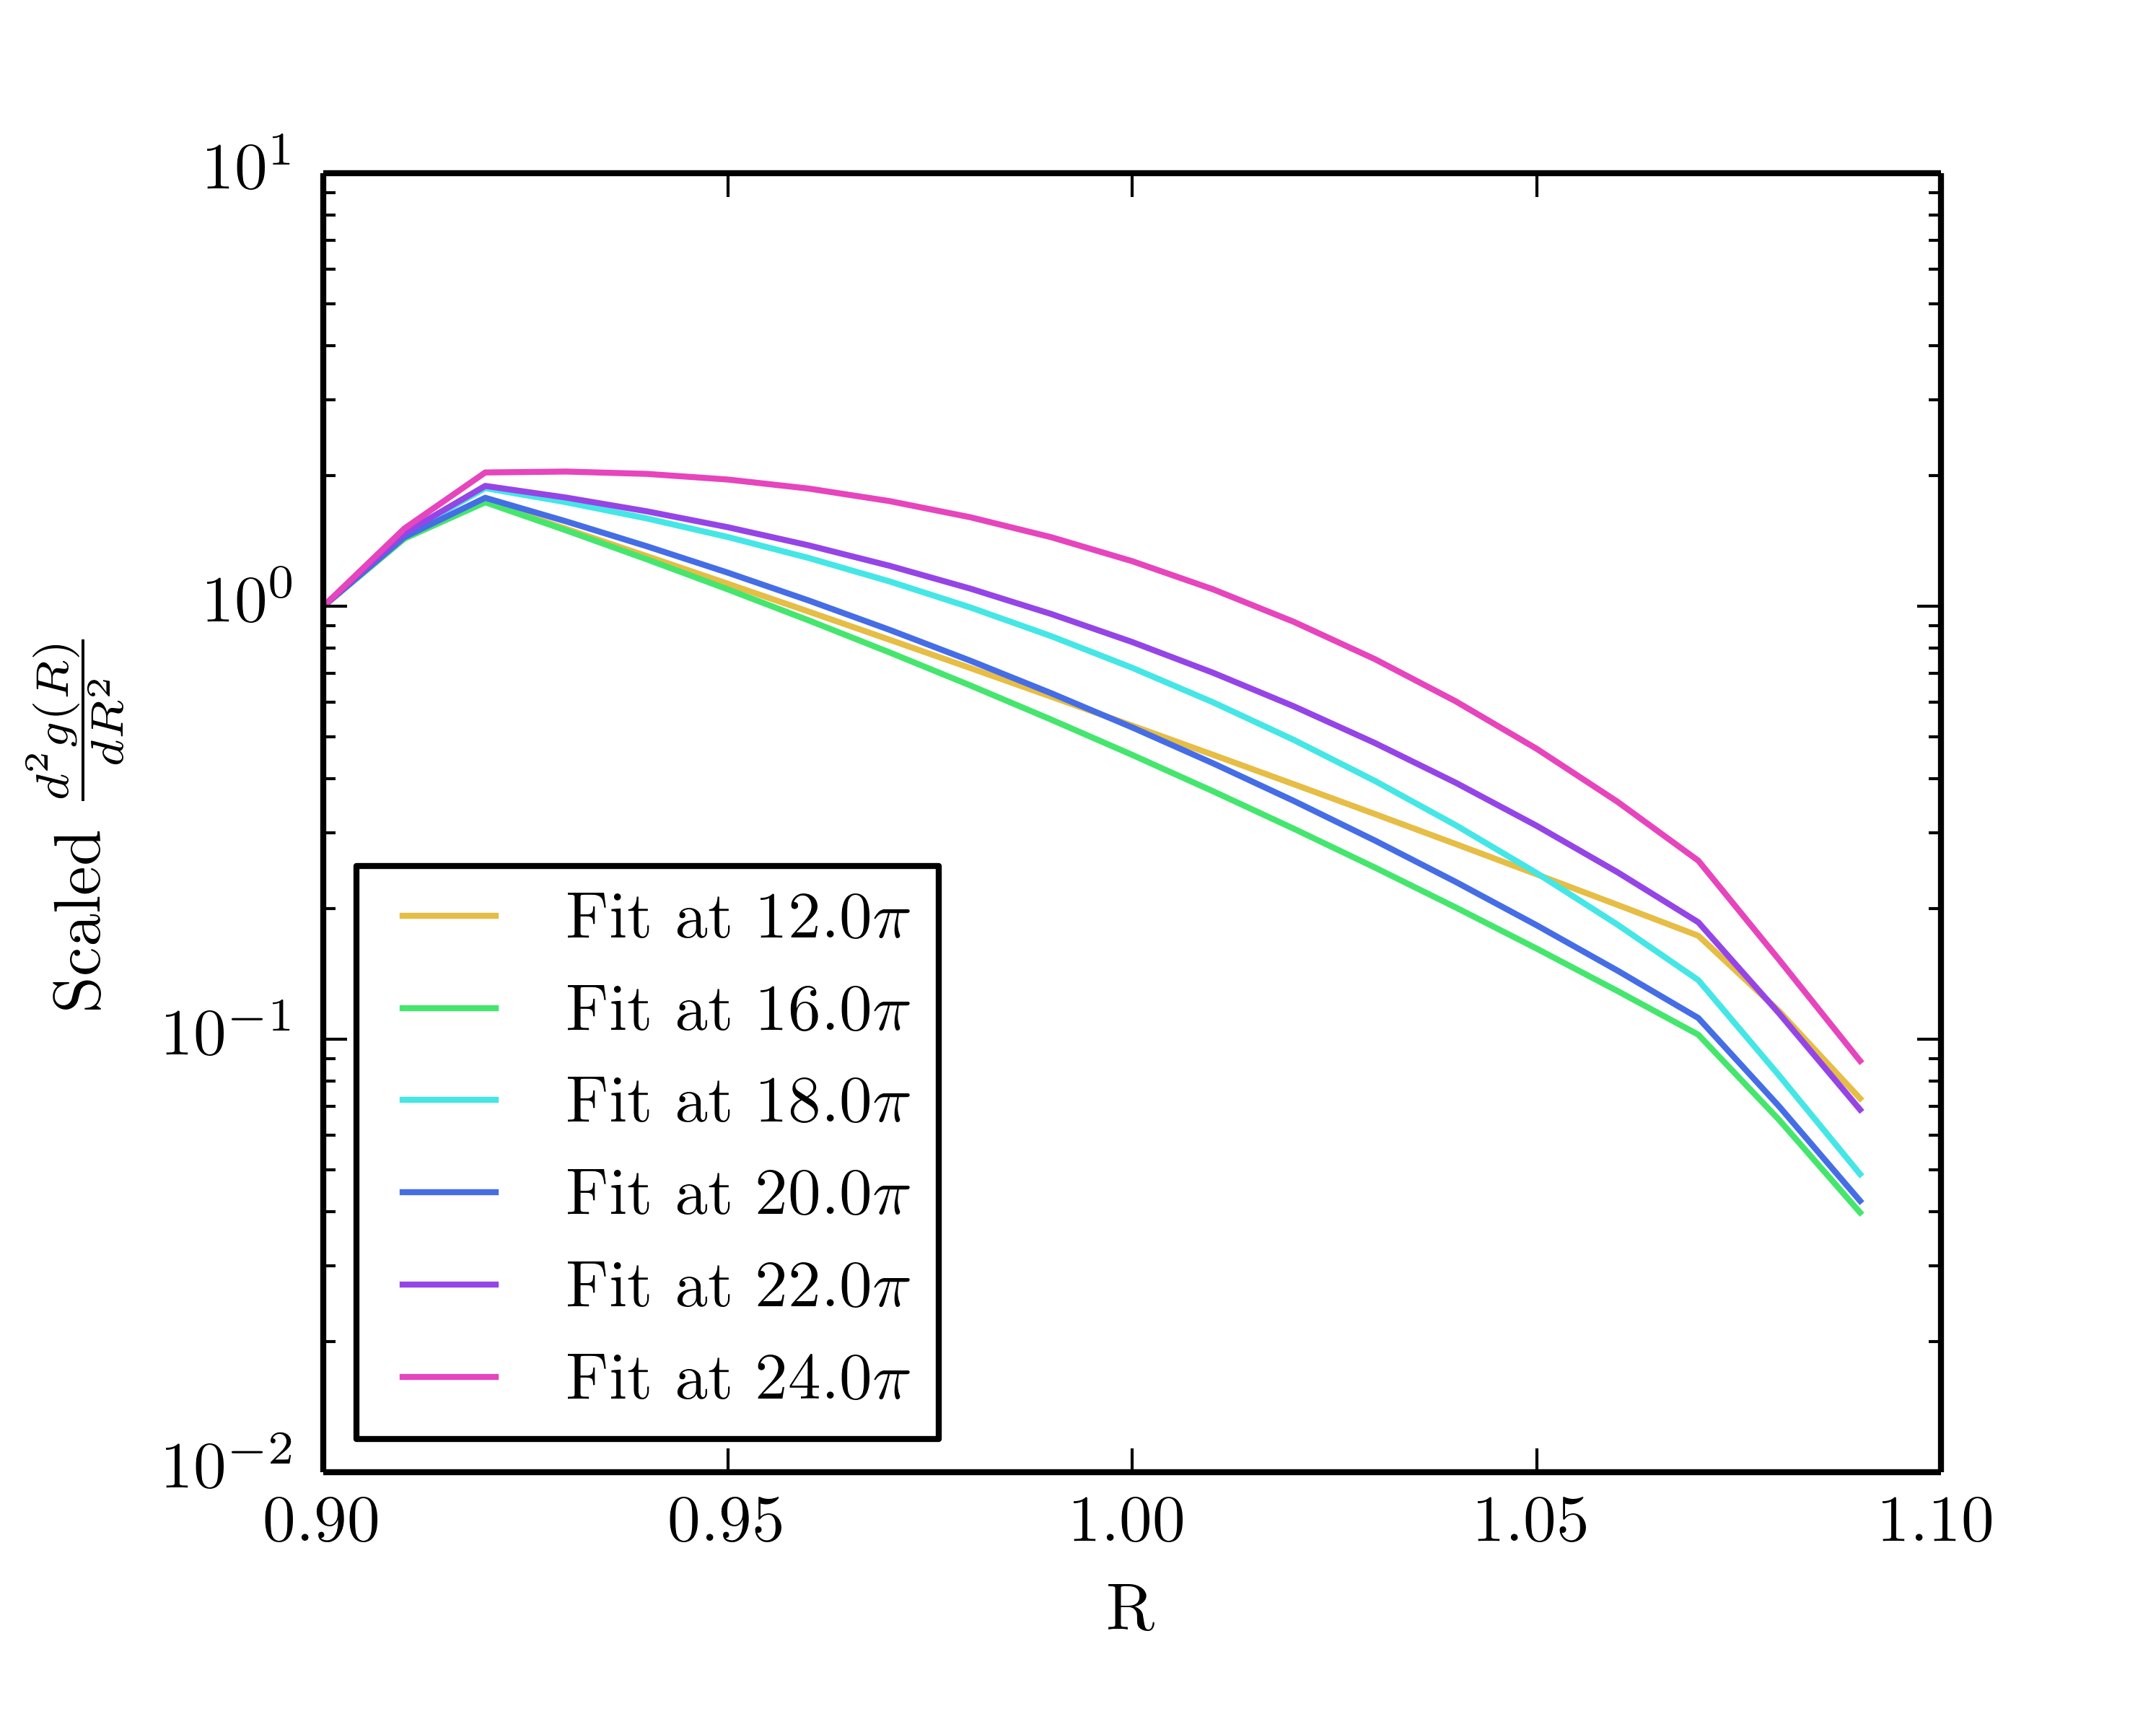
\includegraphics[width=\textwidth]{scaled_fit}
    \caption{Second derivative of \eqref{eq:g} for different domain sizes scaled to the value at $R=0.9$}\label{img:2der}
\end{figure}

As can be seen on Figure~\ref{img:2der}, there does exist a general correlation between the domain size and value of the second derivative, which seems to point towards that conclusion that the motion depends less strongly on $R$ as domain size grows.
For a definitive answer though we would require information on more domain sizes, as well more detailed results at higher $R$s.

\section{Conclusion}

\newpage
\bibliographystyle{plain}
\bibliography{masters}

\newpage
\begin{appendices}
    \section{Program structure}\label{app:struct}
    \subsection{Choice of language}
    Before the start of the project different programming languages were considered for its implementation.
    It was quickly agreed upon that speed and scalability are by far the most important requirements for the program, which left only C++, Haskell and C as the likely contenders (of course only languages familiar to the author were considered).
    We chose C++ against other possibilities, as it has by far the biggest existing code base, good and complete libraries and useful structures for structuring the program in clear fashion.
    One could argue that Haskell provides features of the same or even better quality, but we were substantially less familiar with it and hence it was ruled out.
    Additionally, we feel that through latest additions to the language with the advent of C++11, C++ became a vastly more complete and useful tool.

    \subsection{Modular structure}
    In an effort to keep the code as clear and compartmentalised as possible, we decided to use a runtime plug-in system.
    We were mostly inspired to do so by Rivet\cite{Rivet13} source code, which uses this technique to provide dynamic, runtime-loaded plug-ins for particle analyses.
    On the technical side, our application is divided into a core, which does some initial set-up and fires up the program, and a set of plug-ins.
    The plug-ins are divided into four main groups: \texttt{Computer}s, \texttt{Integrator}s, \texttt{Searcher}s and \texttt{Serializer}s.
    Each of the groups has its own base class, which name is written in a monospaced font above.
    The base class is in charge of some operations common to all instances of the class.
    It provides a common overloadable API, storage and static instance collections.
    Because the API is governed by the base class, in any place in the program where a child class of \texttt{Computer} is used one can substitute this particular child class for any other and no calls will change.
    Additionally, it is possible to retrieve a \texttt{std::list} of available instances of child classes by requesting a static property of one of the base classes called `available'.

    All of these middle-tier base classes inherit from a single templated base class \texttt{Base<T>}.
    The common base reduces code duplication and increases interoperability by supplying boiler-plate code and common overloadble API functions.
    
    \subsubsection{Using the plug-in structure}
    In order to create a new minimal instance of a plug-in child class, one of the middle-tier base classes need to be inherited from.
    At least an implementation of pure virtual functions needs to be provided.
    This still does not enable dynamic runtime discovery of the available plug-ins, which is achieved through calling the registration callback as follows:

    \begin{minted}{c++}
    DECLARE_TURB_PLUGIN(class_name);
    \end{minted}

    Of course \texttt{class\_name} above needs to be substituted with an actual name of the class, \texttt{DECLARE\_TURB\_PLUGIN} needs to be available in current scope (this is achieved by including \textit{helpers.hpp}) and the call should be made outside the \textit{turb} name space.
    This preprocessor macro creates an instance of the current class and shields us from any future changes in the plug-ins architecture.
    Because a new class instance is created to register an instance in the plug-ins manager, it is important to allocate as little memory as possible (preferably none) in a constructor instead deferring memory allocation to another `hook', be it \texttt{allocate}, \texttt{initialize} or something else.

    \subsection{Build system}
    In order to generate portable, state of the art Makefiles, \texttt{CMake} is used.
    It provides us with automatic discovery of available libraries at different locations, intuitive creation of dynamically and statically linked libraries and wide support on target architectures.
    It is also substantially faster in initial preparation than \texttt{automake} and provides progress indication of the compilation, which is greatly helpful with the code longer than few thousands of lines.

    \subsection{Helper programs and scripts}
    \texttt{Bash} and \texttt{Python} are used as scripting languages to help with certain tasks, where appropriate.
    The former is used for streamlining sequences of commands for instance when doing initial set-up of the application.
    The latter turned out to be very useful with generation of batch scripts for running multiple jobs at \texttt{ARCHER} and \texttt{HECToR} and for plot generation.
    At a certain point, before we had access to these supercomputers, scaling was achieved through a rudimentary job system working on \texttt{\href{http://www2.ph.ed.ac.uk/~wjh/faq/}{CPLAB}} computers at the University of Edinburgh.
    This enabled us to run the program at hundreds of cores of virtually unused computers, with full operating system level access to each of them.
    Because of the inability to scale past that quite low amount of cores and a low performance of CPUs, we have obtained the access to the supercomputers and the Python job runner was removed.

    The plots are created in Python using Matplotlib, SciPy and NumPy libraries.
    All the fits used in this thesis are achieved using the same stack, with data caching in Redis where appropriate.
    The ease of using various APIs and wonderful choice of libraries make Python an amazing choice for data analysis.

    The development was conducted with the help of \texttt{git} and \href{https://github.com/mkawalec/masters}{github}.
    Even though all the code was written by the author so none of the collaboration--focused functionality was used, both were very valuable tools for providing backups and edition history.

    \subsection{Libraries used}
    We decided to use as many features available in the core of C++11 as possible, supplementing them with libraries only where needed and found appropriate.
    We have used the \texttt{Boost}\cite{gurtovoy02} library for providing certain needed functionality that could be described as boiler-plate.
    First of all, it enabled us to easily parse command line options.
    We strongly feel that the command line and file options parser implemented in Boost is one of the best ones available for C++.
    Additionally, an architecture-independent nanosecond resolution timer available as a part of Boost has been used for seeding random number generators.
    It is worth noting that we did use an implementation of Mersenne--Twister\cite{Matsumoto98} random number generator from Boost at first, but we decided against it, as the same RNG is available as a part of C++11.

    Because application is usually ran on very big processor counts of above 5000 processors, we needed a data-exchange scheme suitable for such an usage.
    It is provided by \texttt{MPI}\cite{richard06}, which enables virtually perfect scaling of our application, while being acceptably intuitive and clear.
    The biggest power of \texttt{MPI} in our case was that when combined with Run-time Type Information (RTTI) in C++ it is possible to create a framework that facilitates automatic sending of the data using a much more readable API.

    For matrix manipulation, we use a combination of \texttt{Armadillo}\cite{Sanderson10} and a self-written matrix class.
    \texttt{Armadillo} shines when it comes to intuitive usage and a wide range of available operations.
    At certain performance-critical places we use our own matrix structure instead, as it has several benefits.
    First of all it enables ultra-fast row swaps which require only a pointer swap.
    That is achieved while keeping all the data in a continuous block of memory and ensuring that after the swap is applied individual row data is not invalidated in CPU caches.
    Additionally, the data is stored in a row-first manner, which exploits cache locality and memory prefetching when a matrix is multiplied by a vector, resulting in substantially faster multiplications.

    \texttt{Alglib} was used for curve fitting.
    Because fitting done by Alglib was applied at the end of the simulation, we opted to only use the Alglib-created data as a reference and use SciPy curve fitter after the results were retrieved.

    \section{Personal Statement}


\end{appendices}
\end{document}
